
\chapter{Thao tác dữ liệu}
\label{chap:ch3}

\minitoc
\vspace{0.5cm}
\noindent
Trong chương này, ta sẽ xem xét cách máy tính thao tác với dữ liệu và giao tiếp với thiết
bị ngoại vi như máy in và bàn phím. Để làm điều đó, ta sẽ xem xét cơ bản về kiến trúc máy
tính, chỉ ra làm thế nào để lập trình bằng cách mã hoá các lệnh (ở mức máy).


\section{Kiến trúc máy tính}
Phần mạch điện trong máy tính điều khiển các thao tác trên dữ liệu gọi là \textbf{đơn vị
  xử lý trung tâm}, hay CPU - Center Processing Unit.  Người ta thường ví nó như là "bộ
não" của máy tính.
 

Một CPU bao gồm hai phần: \textbf{đơn vị tính toán số học/logic}, hay ALU (viết tắt của
Arthmetic/Logic Unit) và \textbf{đơn vị điều khiển} (control unit). Phần ALU gồm các mạch
thực hiện các phép toán trên dữ liệu (như cộng hoặc trừ). Còn đơn vị điều khiển gồm các
mạch để điều phối các hoạt động của máy. Ngoài ra, để lưu trữ các thông tin trung gian,
CPU còn chứa một tập các ô nhớ, gọi là \textbf{thanh ghi}, tương tự như các ô nhớ của bộ
nhớ chính. Các thanh ghi này được chia làm hai loại: \textbf{thanh ghi đa năng}
(general-purpose registers) và \textbf{thanh ghi chuyên dụng} (special-purpose
registers). Dưới đây, ta xem xét thanh ghi đa năng, còn các thanh ghi chuyên dụng sẽ được
thảo luận trong Mục~\ref{sec:2.3}.

\begin{figure}
  \centering \scalebox{0.6}{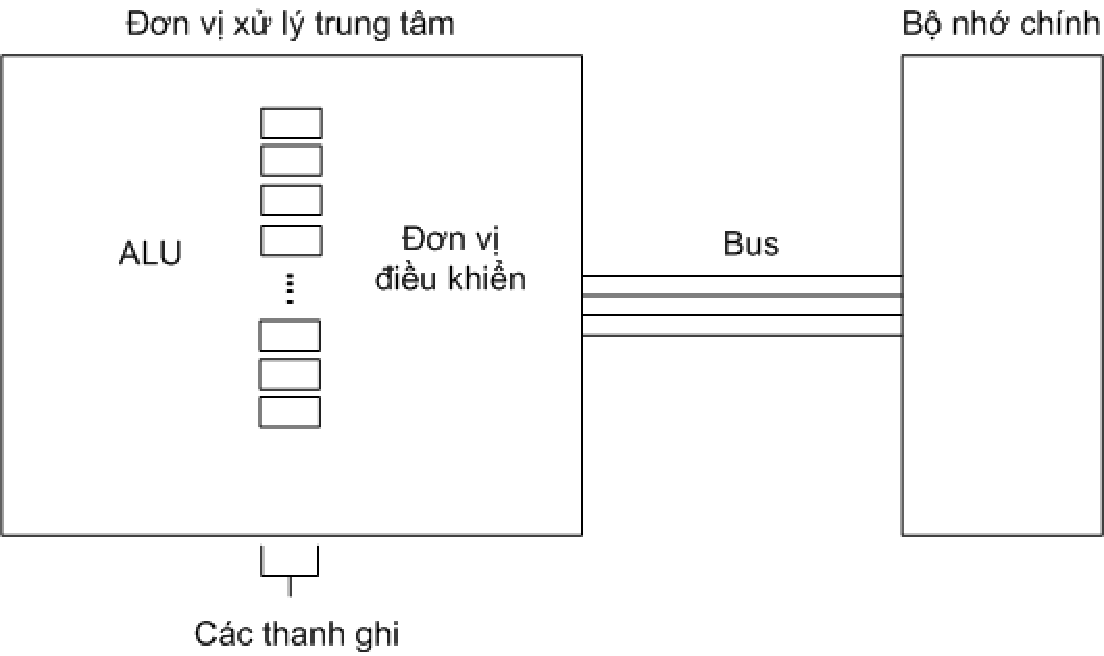
\includegraphics{ch3/fig21.pdf}}
  \caption{CPU và bộ nhớ chính kết nối với nhau thông qua một bus}
  \label{fig:fig21}
\end{figure}

Thanh ghi đa năng dùng để lưu trữ các dữ liệu tạm thời trong khi CPU thực hiện tính
toán. Các thanh ghi này vừa lưu trữ giá trị đầu vào, vừa lưu trữ kết quả sau khi tính toán
của ALU. Để thực hiện một phép toán liên quan đến dữ liệu trong bộ nhớ chính, đơn vị điều
khiển phải chuyển dữ liệu từ bộ nhớ vào các thanh ghi đa năng, thông báo cho ALU biết
thanh ghi nào lưu trữ dữ liệu, kích hoạt mạch thích hợp trong ALU, và thông báo cho ALU
thanh ghi nào để lưu trữ kết quả.      


Để chuyển dữ liệu (dãy bít), CPU và bộ nhớ chính được liên kết với nhau bởi nhiều dây nối,
thường gọi là các \textbf{bus} (xem Hình~\ref{fig:fig21}). Nhờ các bus này, CPU có thể lấy
(đọc) dữ liệu từ bộ nhớ chính bằng cách cung cấp hai thông tin: \begin{inparaenum}[(1)]
\item địa chỉ ô nhớ cần đọc;
\item một tín hiệu đặc biệt thông báo với bộ nhớ gửi dữ liệu cho nó.
\end{inparaenum}
Tương tự, CPU ghi dữ liệu vào bộ nhớ bằng cách cung cấp ba thông
tin: \begin{inparaenum}[(1)]
\item địa chỉ của ô nhớ cần ghi; 
\item dữ liệu cần ghi;
\item một tín hiệu đặc biệt thông báo với bộ nhớ ghi dữ liệu mà nó gửi đến.
\end{inparaenum}

Dựa trên cách thiết kế này, việc cộng hai giá trị nằm trong bộ nhớ chính sẽ không phải chỉ
là thực hiện phép cộng. Thực vậy, để thực hiện thao tác cộng này, nó phải hoàn thành đầy
đủ năm bước liệt kê trong Hình~\ref{fig:fig22}. Tóm lại, các thao tác bao gồm: dữ liệu được
chuyển từ bộ nhớ chính tới các thanh ghi bên trong CPU, sau đó ALU thực hiện cộng giá trị
của các thanh ghi này, và cuối cùng đặt giá trị của thanh ghi kết quả vào trong một ô nhớ
trong bộ nhớ chính.
 
\begin{figure}[tb]
  \centering
  \begin{tabular}{m{1.5cm}m{9cm}}
    Bước $1$. & Lấy toán hạng thứ nhất  từ  trong bộ nhớ và đặt vào các thanh   ghi.\\ \\

    Bước $2$. & Lấy toán hạng thứ hai  từ trong bộ nhớ và đặt nó vào một thanh ghi   khác.   \\  \\

    Bước $3$. & Kích hoạt mạch cộng với đầu vào là các thanh ghi trong các Bước $1$ và
    $2$, và dùng  một thanh ghi khác để lưu kết quả. \\ \\

    Bước $4$. & Lưu giữ kết quả vào trong bộ nhớ. \\ \\

    Bước $5$. & Dừng chương trình. 
  \end{tabular}
  \caption{Cộng các giá trị trong bộ nhớ}
  \label{fig:fig22}
\end{figure}


Các máy tính trước đây rất khó khăn khi thực hiện các công việc khác nhau, vì đối với mỗi
việc, các bước thực hiện phải được xây dựng sẵn trước trong đơn vị điều khiển như một phần
của máy. Để có được tính mềm dẻo, các thiết bị điện trước đây được thiết kế sao cho có thể
dễ dàng nối lại dây tương ứng cho mỗi nhiệm vụ. Trước khi thực hiện một nhiệm vụ các dây
nối phải được cắm sẵn vào trong các lỗ cắm thích hợp. Cách thiết kế này giống như chuyển
mạch trong các hệ thống điện thoại đời cũ.

Mọi vấn đề được giải quyết nhờ vào ý tưởng mang tính đột phá của Von Neumann. Ông đã chỉ
ra rằng chương trình cũng là một loại dữ liệu, nó được mã hoá và lưu trong bộ nhớ
chính. Nếu đơn vị điều khiển được thiết kế để đọc lệnh từ bộ nhớ, giải mã lệnh, và thực
hiện lệnh, thì thay vì phải nối lại dây để thay đổi chương trình máy tính, ta chỉ phải đặt
nội dung của một vài ô nhớ tương ứng với chương trình.

Ý tưởng về chương trình được đặt trong bộ nhớ chính được gọi là \textbf{khái niệm lưu trữ
  chương trình}. Ngày nay, nó trở thành cách tiếp cận chính thống - nó quen thuộc tới mức
đã trở nên hiển nhiên trong việc thiết kế máy tính. Thực chất, những khó khăn của thời kỳ
trước là do mọi người đã quen với việc phân biệt chương trình và dữ liệu như những thực
thể khác nhau: dữ liệu được lưu trữ trong bộ nhớ, còn chương trình phải là một phần của
đơn vị điều khiển. Đây là một ví dụ điển hình cho thấy lợi ích khi thay đổi cách tư duy.

\subsection*{Câu Hỏi \& Bài tập}

\begin{enumerate}
\item Bạn hãy chỉ ra dãy các hoạt động cần thiết để chuyển dữ liệu từ một ô nhớ này tới
  một ô nhớ khác trong máy tính?

\item Để có thể ghi một giá trị vào ô nhớ, CPU phải cung cấp cho bộ nhớ chính những thông
  tin gì?

\item Thiết bị lưu trữ khối, bộ nhớ chính, và thanh ghi đa năng đều là các hệ thống lưu
  trữ. Hãy chỉ ra sự khác nhau trong cách sử dụng của chúng?

\end{enumerate}

\section{Ngôn ngữ máy}
Để áp dụng được khái niệm lưu trữ chương trình, các CPU được thiết kế để đoán nhận các
lệnh được mã hoá dưới dạng các dãy bít. Tập các lệnh cùng với cách mã hoá được gọi là
\textbf{ngôn ngữ máy}. Các lệnh biểu thị trong ngôn ngữ này được gọi là lệnh ở mức máy,
hay ngắn gọn là \textbf{lệnh máy}.

\subsection*{Tập lệnh}
Danh sách các lệnh mà một CPU điển hình có thể giải mã và thực hiện được khá ngắn. Khi mà
một máy đã có thể thực hiện một số nhiệm vụ cơ bản và được lựa chọn hợp lý, việc thêm vào
một số đặc điểm, về mặt lý thuyết, sẽ không làm tăng khả năng của máy. Nói cách khác, việc
thêm những đặc điểm này chỉ làm máy thêm thích hợp với người sử dụng, chứ không tăng chức
năng cơ bản của nó.

Có hai quan điểm về kiến trúc CPU. Một quan điểm cho rằng CPU nên được thiết kế chỉ có một
số tối thiểu các lệnh máy cần thiết. Cách tiếp cận này dẫn tới khái niệm \textbf{kiến trúc
  tập lệnh rút gọn} (RISC - reduced instruction set computer). Ưu điểm của kiến trúc RISC
là máy thực hiện hiệu quả và nhanh chóng do tính đơn giản của tập lệnh.

Quan điểm khác cho rằng CPU nên có sẵn một tập lớn các lệnh phức tạp, dù chúng có dư thừa
về mặt kỹ thuật. Kết quả cách tiếp cận này là \textbf{kiến trúc tập lệnh phức tạp} (CISC -
reduced instruction set computer).  Luận điểm của kiến trúc CISC là nếu CPU phức tạp có
nghĩa là việc viết chương trình trên đó sẽ đơn giản.  Bởi vậy, để thực hiện một lệnh phức
tạp ở kiến trúc CISC nói chung cần thực hiện nhiều lệnh ở kiến trúc RISC.

Cả hai loại bộ xử lý RISC và CISC đều có sẵn trên thị trường. Dòng xử lý Pentium, được
phát triển bởi Intel, là một ví dụ về kiến trúc CISC. Dòng PowerPC (bao gồm các bộ xử lý
mà Apple gọi là G4 và G5), được phát triển bởi Apple, IBM và Motorola là ví dụ về kiến
trúc RISC.  (Apple hiện nay sản xuất máy dựa trên sản phẩm của Intel. Tuy nhiên, việc
chuyển đổi này là vì lý do thương mại, chứ không phải là do phân biệt ưu nhược điểm của
triết lý thiết kế RISC và CISC).

Dù ở kiến trúc RISC hay CISC, một lệnh máy vẫn có thể được phân loại thành ba
nhóm: \begin{inparaenum}[(1)]
\item nhóm lệnh chuyển dữ liệu;
\item nhóm lệnh số học và logic;
\item nhóm lệnh điều khiển.
\end{inparaenum}

\paragraph{Chuyển dữ liệu} Nhóm chuyển dữ liệu bao gồm các lệnh yêu cầu chuyển dữ liệu từ
ô nhớ này sang ô nhớ khác. Các bước 1, 2, và 4 trong Hình \ref{fig:fig22} là loại lệnh
này. Ta nên để ý rằng việc sử dụng thuật ngữ \textit{chuyển} ở đây không hoàn toàn chính
xác. Rất hiếm khi dữ liệu được chuyển đi bằng cách sao chép sang ô nhớ mới đồng thời xoá ở
ô nhớ gốc. Lệnh chuyển ở đây giống như việc sao chép dữ liệu hơn. Bởi vậy nên mô tả hoạt
động của nhóm lệnh này bằng thuật ngữ sao chép thay vì chuyển.

Cũng liên quan đến thuật ngữ, ta thảo luận hai thuật ngữ đặc biệt thường dùng cho thao tác
chuyển dữ liệu giữa CPU và bộ nhớ chính: đó là LOAD và STORE. Yêu cầu đặt giá trị cho
thanh ghi đa năng bằng nội dung của ô nhớ thường được gọi là lệnh LOAD.  Ngược lại, yêu
cầu chuyển nội dung của thanh ghi vào trong một ô nhớ được gọi là STORE. Trong hình
\ref{fig:fig22}, Bước 1 và 2 là lệnh LOAD, và bước 4 là lệnh STORE.

Một nhóm con quan trọng trong nhóm lệnh chuyển dữ liệu là các lệnh giao tiếp với thiết bị
ngoại vi (như máy in, bàn phím, màn hình, bộ điều khiển đĩa,...). Bởi vì các lệnh này thực
hiện các hoạt động vào/ra (I/O) của máy, nên chúng được gọi là lệnh I/O. Thực chất, các
lệnh này được thực hiện nhờ vào các lệnh chuyển dữ liệu giữa CPU và bộ nhớ, ta sẽ giải
thích chi tiết cách làm trong Mục~\ref{sec:2.5}. Vì vậy, ta cũng xếp các lệnh I/O vào nhóm
lệnh chuyển dữ liệu.

\paragraph{Số học và logic} Nhóm số học và logic gồm các lệnh nhằm thông báo với bộ điều
khiển yêu cầu một hoạt động xử lý bởi đơn vị tính toán số học và logic. Bước 3 trong hình
\ref{fig:fig22} rơi vào nhóm này. Giống như tên gọi, đơn vị số học và logic không chỉ có khả
năng thực hiện các phép toán số học, mà còn nhiều phép toán khác nữa.  Một số trong đó là
các phép toán Boolean $\AND$, $\OR$ và $\XOR$ như được giới thiệu trong Chương~\ref{chap:chuong1}.

Ngoài ra, một tập các phép toán khác sẵn có trong hầu hết các đơn vị số học và logic cho
phép dịch nội dung thanh ghi sang phải hoặc trái. Các phép toán này được biết như các phép
toán SHIFT hoặc ROTATE. Sự khác biệt giữa hai lệnh này là, đối với lệnh SHIFT thì bít ``ở
vị trí cuối cùng'' của thanh ghi bị bỏ qua, còn với ROTATE thì bít này được quay vòng lại
phía đầu bên kia của thanh ghi.

\paragraph{Điều khiển} Nhóm lệnh điều khiển bao gồm các lệnh trực tiếp thực hiện chương
trình thay vì thao tác dữ liệu. Bước 5 trong Hình \ref{fig:fig22} thuộc nhóm lệnh
này. Nhóm lệnh này chứa nhiều lệnh rất quan trọng trong tập lệnh máy, như họ các lệnh nhảy
JUMP (hoặc BRANCH) được sử dụng để thay đổi thứ tự thực hiện lệnh. Nó cho phép chuyển đến
thực hiện một lệnh bất kỳ, thay vì thực hiện lệnh tiếp theo trong danh sách lệnh. Có hai
kiểu lệnh JUMP: \textbf{lệnh nhảy không điều kiện} và \textbf{lệnh nhảy có điều kiện}. Một
ví dụ của kiểu lệnh nhảy không điều kiện là ``Nhảy tới Bước 5''; một ví dụ của kiểu lệnh
nhảy có điều kiện là ``Nếu giá trị đạt được là 0, vậy nhảy tới Bước 5''. Sự khác biệt giữa
các lệnh này là lệnh nhảy có điều kiện thực hiện ``thay đổi nơi đến'' chỉ nếu một số điều
kiện được thoả mãn. Như một ví dụ, dãy các lệnh trong Hình~\ref{fig:fig23} biểu diễn thuật
toán chia hai giá trị ở đó Bước 3 là điều kiện nhảy có điều kiện nhằm tránh trường hợp
chia cho không.

\begin{figure}[tb]
  \begin{center}
    \begin{tabular}{m{2cm}m{7cm}}
      Bước $1$. & LOAD một thanh ghi với một giá trị từ bộ nhớ.         \\   \\

      Bước $2$. & LOAD thanh ghi khác với giá trị khác trong bộ nhớ.    \\   \\

      Bước $3$. & Nếu giá trị thứ hai này bằng không,                   \\
      & JUMP tới Bước $6$.                                    \\   \\

      Bước $4$. & Chi nội dung của thanh ghi đầu tiên với thanh ghi thứ hai   và đặt kết quả vào thanh ghi thứ ba.                              \\   \\

      Bước $5$. & STORE nội dung của thanh ghi thứ ba vào trong bộ nhớ. \\   \\

      Bước $6$. & STOP.
    \end{tabular}
  \end{center}
  \caption{Chia các giá trị trong bộ nhớ}
  \label{fig:fig23}

\end{figure}

\subsection*{Một mô tả ngôn ngữ máy}
Ta sẽ cùng xem xét cách mã hoá các lệnh của một máy tính. Máy mà ta sẽ sử dụng cho thảo
luận sẽ được mô tả trong Phụ lục~\ref{phuluc1} và được tóm tắt trong
Hình~\ref{fig:fig24}. Máy này gồm~$16$ thanh ghi đa năng và bộ nhớ chính gồm $256$ ô nhớ,
mỗi ô nhớ có khả năng lưu trữ tám bít. Để tiện tham chiếu, ta gán nhãn các thanh ghi bởi
các giá trị từ $0$ tới $15$ và địa chỉ của các ô nhớ từ $0$ tới $255$. Để tiện lợi, ta xem
các nhãn và địa chỉ này như các giá trị nhị phân và viết gọn dưới dạng hexa. Và do đó, các
thanh ghi được gán nhãn từ $0$ tới $F$, và các ô nhớ được đánh địa chỉ từ $00$ tới $FF$.

\begin{figure}[tbh]
  \centering \scalebox{0.6}{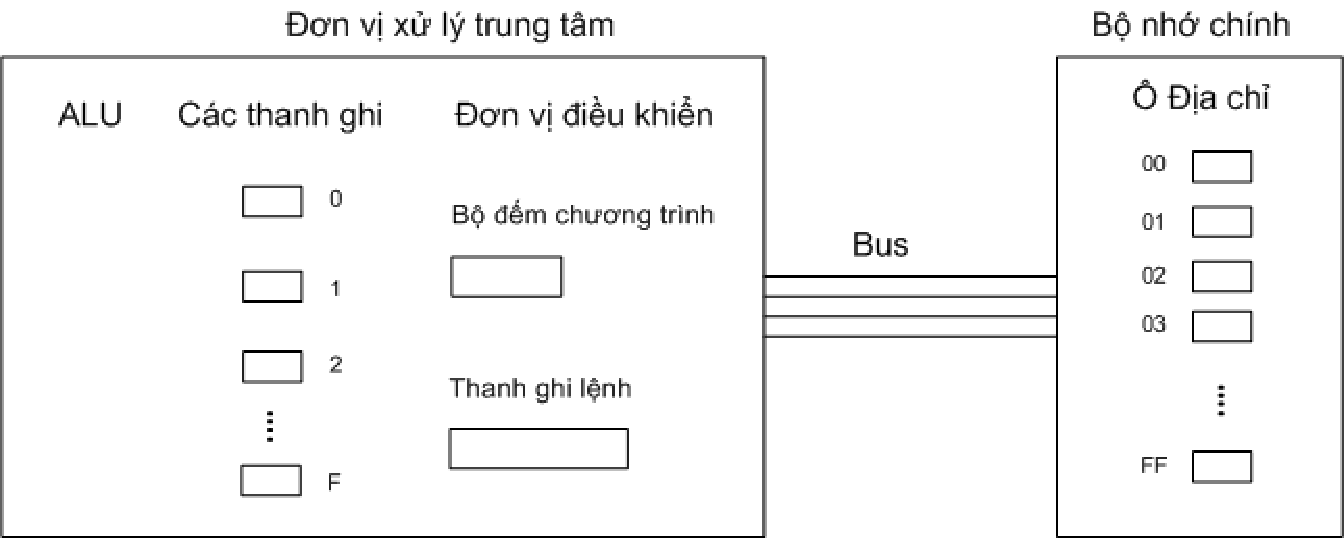
\includegraphics{ch3/fig24.pdf}}
  \caption{Kiến trúc máy được mô tả trong Phụ lục \ref{phuluc1}}
  \label{fig:fig24}
\end{figure}

Các lệnh máy được mã hoá gồm hai phần: trường \textbf{op-code} (viết tắt của mã toán tử)
và trường \textbf{toán hạng}. Dãy bít xuất hiện trong phần op-code chỉ ra phép toán nào
được thực hiện, kiểu như STORE, SHIFT, XOR, và JUMP; và trường này bắt buộc phải có trong
mọi lệnh. Dãy bít trong trường toán hạng cung cấp các thông tin chi tiết về phép toán được
xác định bởi op-code. Ví dụ với phép toán STORE, thông tin trong trường toán hạng chỉ
ra: \begin{inparaenum}[(1)]
\item thanh ghi nào chứa dữ liệu cần ghi;
\item và ô nhớ nào để nhận dữ liệu. 
\end{inparaenum}

Ngôn ngữ máy mô tả ở Phục lục \ref{phuluc1} chỉ gồm $12$ lệnh cơ bản. Mỗi lệnh được mã hoá
bằng $16$ bít, và biểu diễn bởi một số thập lục phân gồm bốn chữ số
(Hình~\ref{fig:fig25}). Trong đó, bốn bít đầu tiên là phần op-code, hay tương đương chữ số
dầu tiên của số thập lục phân. Để ý (Phụ lục \ref{phuluc1}) rằng các op-code này được biểu
diễn bởi các chữ số hexa từ $1$ tới~$C$. Đặc biệt, Bảng trong Phụ lục \ref{phuluc1} chỉ
cho ta rằng một lệnh bắt đầu bằng chữ số $3$ (ở dạng hexa) tham chiếu đến lệnh STORE, lệnh
bắt đầu bằng chữ số $A$ tham chiếu đến lệnh ROTATE.

\begin{figure}[bth] 
  \centering \input{ch3/fig25}
  \caption{Các thành phần của một lệnh máy trong Phụ lục \ref{phuluc1}}
  \label{fig:fig25}
\end{figure}


Trường toán hạng của mỗi lệnh trong mô tả máy của ta bao gồm ba chữ số hexa~(12 bít), và
ngoại trừ lệnh HALT không cần thông tin gì thêm, nó sẽ làm rõ xem lệnh đưa bởi op-code
phải làm gì. Ví dụ, xem Hình~\ref{fig:fig26}, nếu chữ số hexa đầu tiên của một lệnh là $3$
chỉ ra đây là lệnh lưu trữ nội dung của thanh ghi vào bộ nhớ, số hexa tiếp theo của lệnh
chỉ ra thanh ghi nào cần lưu trữ, và hai số hexa cuối chỉ ra ô nhớ nào dùng để lưu dữ
liệu. Bởi vậy lệnh $35A7$ (ở dạng hexa) dịch thành lệnh ``STORE mẫu bít tìm thấy trong
thanh ghi 5 vào trong ô nhớ có địa chỉ là A7''. Chú ý rằng việc sử dụng ký hiệu hexa giúp
ta đơn giản trong việc nhìn các lệnh. Còn trên thực tế, lệnh $35A7$ là dãy
bít~$0011010110100111$.
 

%\begin{wrapfigure}{r}{90mm}
\begin{figure}[thb]
  \centering \input{ch3/fig26}
  \caption{Giải mã lệnh $35A7$}
  \label{fig:fig26}
\end{figure}
%\end{wrapfigure}

Lệnh $35A7$ cũng cung cấp một ví dụ rõ ràng tại sao dung lượng bộ nhớ chính được tính theo
luỹ thừa của hai. Bởi vì tám bít trong lệnh để dành cho việc xác định ô nhớ nào được sử
dụng trong lệnh, nó có khả năng tham khảo tới chính xác $2^8$ ô nhớ khác nhau. Bởi thế ta
cần xây dựng bộ nhớ có đúng số ô nhớ như thế--đánh địa chỉ từ $0$ tới $255$. Nếu bộ nhớ
chính có nhiều ô nhớ hơn, thì số ta không thể viết lệnh phân biệt chúng; còn nếu có ít ô
nhớ hơn, có trường hợp ta viết lệnh tham chiếu đến một ô nhớ không tồn tại.


Một ví dụ khác chỉ ra xem làm thế nào trường toán hạng được sử dụng để làm rõ lệnh xác
định bởi op-code. Ta xét lệnh có op-code $7$ (ở dạng hexa), lệnh này yêu cầu $\OR$ nội
dung của hai thanh ghi với nhau (ta sẽ giải thích làm thế nào để $\OR$ hai thanh ghi sau,
trong Mục~\ref{sec:2.4}). Bây giờ ta chỉ đơn thuần quan tâm xem làm thế nào lệnh được mã
hoá. Trong trường hợp này, chữ số hexa tiếp theo chỉ ra thanh ghi nào sẽ được lưu kết quả,
còn hai số hexa cuối chỉ ra hai thanh ghi nào sẽ được $\OR$ với nhau. Bởi vậy lệnh~$70C5$
được dịch thành ``OR nội dung của thanh ghi $C$ với nội dung của thanh ghi $5$ và đặt kết
quả vào thanh ghi $0$''.

Ta cũng cần phân biệt giữa hai lệnh máy LOAD. Ở đây ta, lệnh có op-code $1$ (ở dạng hexa)
là lệnh nạp giá trị là nội dung của một ô nhớ vào một thanh ghi, trong khi đó op-code $2$
(ở dạng hexa) là lệnh nạp một hằng số vào thanh ghi. Sự khác biệt ở đây là, với lệnh nạp
kiểu đầu tiên, trường toán hạng chứa một địa chỉ; trong khi đó, với lệnh nạp kiểu thứ hai,
trường toán hạng là dãy bít cần được được nạp.

Để ý rằng máy có hai lệnh ADD, một để cộng hai số biểu diễn bù hai và một để cộng biểu
diễn dấu chấm động. Sự phân biệt này là hậu quả của sự kiện rằng, bên trong đơn vị số học
và logic, cách hoạt động để cộng các số được mã hoá ở dạng bù hai khác với cách cộng các
số mã hoá theo ký hiệu dấu chấm động .

\begin{figure}[thb]
  \centering
  \begin{tabular}{m{2.5cm}m{7cm}}
    \textbf{Lệnh}   & \textbf{Ý nghĩa}                                                             \\ \\
    $156C$ & Nạp thanh ghi $5$ với giá trị bằng với xâu bít tìm thấy trong bộ nhớ tại địa chỉ $6C$                                                                           \\ \\

    $166D$ & Nạp thanh ghi $6$ bằng xâu bít tìm thấy tại ô nhớ có địa chỉ là $6D$. \\  \\

    $5056$ & Cộng nội dung biểu diễn dưới dạng bù hai của thanh ghi $5$ và thanh ghi $6$ và lưu kết quả vào thanh ghi  $0$.                                                \\ \\

    $306E$ & Lưu nội dung của thanh ghi $0$ vào trong bộ nhớ tại địa chỉ $6E$.     \\ \\

    $C000$ & Dừng chương trình. 
  \end{tabular}
  \caption{Một cách mã hoá các lệnh trong Hình~\ref{fig:fig22}}
  \label{fig:fig27}
\end{figure}


Ta kết thúc phần này với Hình~\ref{fig:fig27}, nó chứa mã một cách mã hoá của lệnh trong hình
\ref{fig:fig22}. Ta giả sử rằng các giá trị được cộng đã được lưu trữ như các số bù hai tại ô
nhớ có địa chỉ $6C$ và $6D$ và tổng của chúng sẽ được đặt tại địa chỉ $6E$.

\subsection*{Câu Hỏi \& Bài Tập}
\begin{enumerate}
\item Tại sao thuật ngữ \textit{dịch chuyển} (move) được xem như một tên không đúng cho
  phép toán dịch chuyển dữ liệu từ một vị trí tới một vị trí khác trong máy?

\item Trong phần trình bày ở trên, các lệnh JUMP đã được giải thích bằng cách xác định rõ
  rằng vị trí nhảy tới bởi tên (hoặc số bước nhảy) của lệnh đích bên trong lệnh JUMP (ví
  dụ, ``Nhảy tới Bước 6''). Một trở ngại của cách tiếp cận này là nếu tên một lệnh (số) bị
  thay đổi sau đó, ta sẽ phải tìm được mọi lệnh nhảy tới lệnh đó và thay đổi lại phần tên
  trong lệnh. Hãy mô tả một cách khác giải thích lệnh JUMP sao cho tên lệnh đích không cần
  phải xác định một cách rõ ràng.

\item Lệnh ``Nếu $0$ bằng $0$, thì nhảy tới Bước $7$'' là lệnh nhảy có điều kiện hay không
  có điều kiện? Giải thích câu trả lời của bạn.

\item Viết lại chương trình trong Hình \ref{fig:fig27} dưới dạng các dãy bít.

\item Các lệnh sau đây được viết trong ngôn ngữ máy mô tả ở Phụ lục \ref{phuluc1}. Hãy mô
  tả chính xác chúng bằng ngôn ngữ tự nhiên.

  \begin{inparaenum}[a. ]
  \item $386A$ \qquad \qquad \qquad
  \item $BADE$ \qquad \qquad \qquad
  \item $803C$ \qquad \qquad \qquad
  \item $40F4$
  \end{inparaenum}

\item Nêu sự khác nhau giữa các lệnh $15AB$ và $25AB$ trong ngôn ngữ máy mô tả ở Phụ lục
  \ref{phuluc1}.

\item Dưới đây là mộ tả của một vài lệnh. Hãy dịch chúng sang ngôn ngữ máy trong Phụ lục
  \ref{phuluc1}.
  \begin{enumerate}
  \item LOAD thanh ghi số $3$ với giá trị hexa là $56$.

  \item ROTATE thanh ghi số $5$ ba bít sang phải.

  \item AND nội dung của thanh ghi $A$ với nội dung của thanh ghi $5$ và đặt kết quả vào
    thanh ghi $0$.
  \end{enumerate}
\end{enumerate}

\section{Thực hiện chương trình}
\label{sec:2.3}


Máy tính thực hiện một chương trình nằm trong bộ nhớ bằng cách sao chép các lệnh vào đơn
vị điều khiển. Tại đơn vị điều khiển, từng lệnh một được giải mã và thực thi. Thứ tự các
lệnh được nạp từ bộ nhớ tương ứng với thứ tự chúng được lưu trữ trong bộ nhớ, trừ trường
hợp lệnh hiện hành được chọn trước đó bởi một lệnh nhảy~JUMP.

Để hiểu quá trình này hoạt động thế nào, ta cần phải xem xét tổ chức của đơn vị điều khiển
trong CPU. Nó có hai thanh ghi chuyên dụng: \textbf{thanh ghi lệnh} và \textbf{bộ đếm
  chương trình} (xem lại Hình~\ref{fig:fig24}). Thanh ghi lệnh lưu giữ lệnh đang thực
hiện. Bộ đếm chương trình chứa địa chỉ của lệnh tiếp theo sẽ được thực hiện; bằng cách
này, máy biết được lệnh tiếp theo nó sẽ phải thực hiện là lệnh gì.

%\begin{wrapfigure}{r}{60mm}
\begin{figure}[tbh]
  \begin{center}
    \input{ch3/fig28}
  \end{center}
  \caption{Chu kỳ máy}
  \label{fig:fig28}
\end{figure}
%\end{wrapfigure}
Đơn vị điều khiển thực hiện lệnh theo một quá trình gồm ba bước, gọi là \textbf{chu kỳ
  máy}.  Các bước này gồm: nạp, giải mã, và thực hiện lệnh (Hình~\ref{fig:fig28}). Trong
bước nạp, đơn vị điều khiển yêu cầu bộ nhớ cung cấp cho nó lệnh được lưu trữ tại ô nhớ
được chỉ ra bởi bộ đếm chương trình. Bởi vì mỗi lệnh trong máy bao gồm $2$ byte, bước nạp
sẽ lấy nội dung của hai ô nhớ liên tiếp từ bộ nhớ chính. Nó đặt hai ô nhớ này vào thanh
ghi lệnh như một lệnh, sau đó tăng bộ đếm chương trình lên hai để trỏ tới lệnh tiếp
theo. Như vậy, bộ đếm chương trình đã sẵn sàng cho bước nạp tiếp theo.

Khi lệnh đã nằm trong thanh ghi lệnh, đơn vị điều khiển tiến hành giải mã để tách riêng
từng toán hạng tương ứng với từng thành phần của lệnh dựa trên phần op-code của nó. Sau
đó, đơn vị điều khiển sẽ thực hiện lệnh bằng cách kích hoạt các mạch điện phù hợp với
nhiệm vụ được yêu cầu. Ví dụ, nếu là lệnh nạp dữ liệu từ bộ nhớ, đơn vị điều khiển sẽ gửi
tín hiệu tương ứng tới bộ nhớ chính, đợi bộ nhớ chính gửi lại dữ diệu, và đưa dữ liệu nhận
được vào các thanh ghi được yêu cầu. Nếu lệnh cần thực hiện đòi hỏi tính toán số học, đơn
vị điều khiển sẽ kích hoạt mạch điện thích hợp của đơn vị số học và logic với các thanh
ghi đầu vào thích hợp; đợi câu trả lời từ đơn vị tính toán số học và logic để đặt vào các
thanh ghi đầu ra được yêu cầu.

Khi lệnh ở trong thanh ghi lệnh đã thực hiện xong, đơn vị điều khiển lại bắt đầu chu kỳ
máy mới. Để ý rằng bộ đếm chương trình đã được tăng ở cuối mỗi bước nạp, vậy nó trỏ đến
địa chỉ lệnh đúng cho bước nạp của chu kỳ sau.

\begin{figure}  
  \centering \input{ch3/fig29}
  \caption{Giải mã lệnh $B258$}
  \label{fig:fig29}
\end{figure}

Có gì đặc biệt khi thực hiện lệnh nhảy JUMP? Ta xem xét, ví dụ lệnh $B258$
(Hình~\ref{fig:fig29}), ý nghĩa của nó là ``JUMP tới lệnh tại địa chỉ $58$ (dạng hexa) nếu
nội dung của thanh ghi~$2$ bằng với nội dung thanh ghi $0$''. Trong trường hợp này, ở bước
thực hiện của chu kỳ máy, đầu tiên máy sẽ tiến hành so sánh nội dung hai thanh ghi $2$ và
$0$. Nếu chúng là hai dãy bít khác nhau, bước thực hiện kết thúc và chu kỳ máy tiếp theo
sẽ bắt đầu. Ngược lại, nếu nội dung của hai thanh ghi này bằng nhau, máy sẽ đặt giá trị
$58$ (dạng hexa) vào bộ đếm chương trình (vẫn trong bước thực hiện). Trong trường hợp này,
bước nạp tiếp theo sẽ thấy $58$ trong bộ đếm chương trình, và lệnh tiếp theo sẽ tại địa
chỉ này sẽ được nạp và thực hiện.

Chú ý rằng, nếu lệnh là $B058$, vậy thì việc quyết định khi nào bộ đếm chương trình bị
thay đổi sẽ phụ thuộc vào khi nào nội dung thanh ghi $0$ bằng nội dung thanh ghi $0$. Vậy
thì, đây là lệnh nhảy không điều kiện. Và mọi lệnh có dạng $B0xy$ sẽ thực hiện nhảy tới vị
trí $xy$ mà không cần quan tâm đến nội dung của thanh ghi~$0$.

\subsection*{Một ví dụ về quá trình thực hiện chương trình}
Ta sẽ thử áp dụng các thảo luận về chu kỳ máy ở trên cho chương trình trong
Hình~\ref{fig:fig27}. Chương trình này nạp hai giá trị từ bộ nhớ chính, tính toán tổng của
chúng, và ghi lại vào một ô nhớ trong bộ nhớ. Đầu tiên ta cần đặt chương trình vào một nơi
trong bộ nhớ. Trong ví dụ này, ta giả sử chương trình đã được lưu giữ tại vùng nhớ liên
tục bắt đầu tại địa chỉ $A0$ (hexa). Khi chương trình đã được lưu trữ theo cách này, ta có
thể chạy chương trình bằng cách đặt địa chỉ ($A0$) của lệnh đầu tiên trong bộ đếm chương
trình và cho máy chạy (Hình \ref{fig:fig210}).

\begin{figure}[tbh]
  \centering \scalebox{0.6}{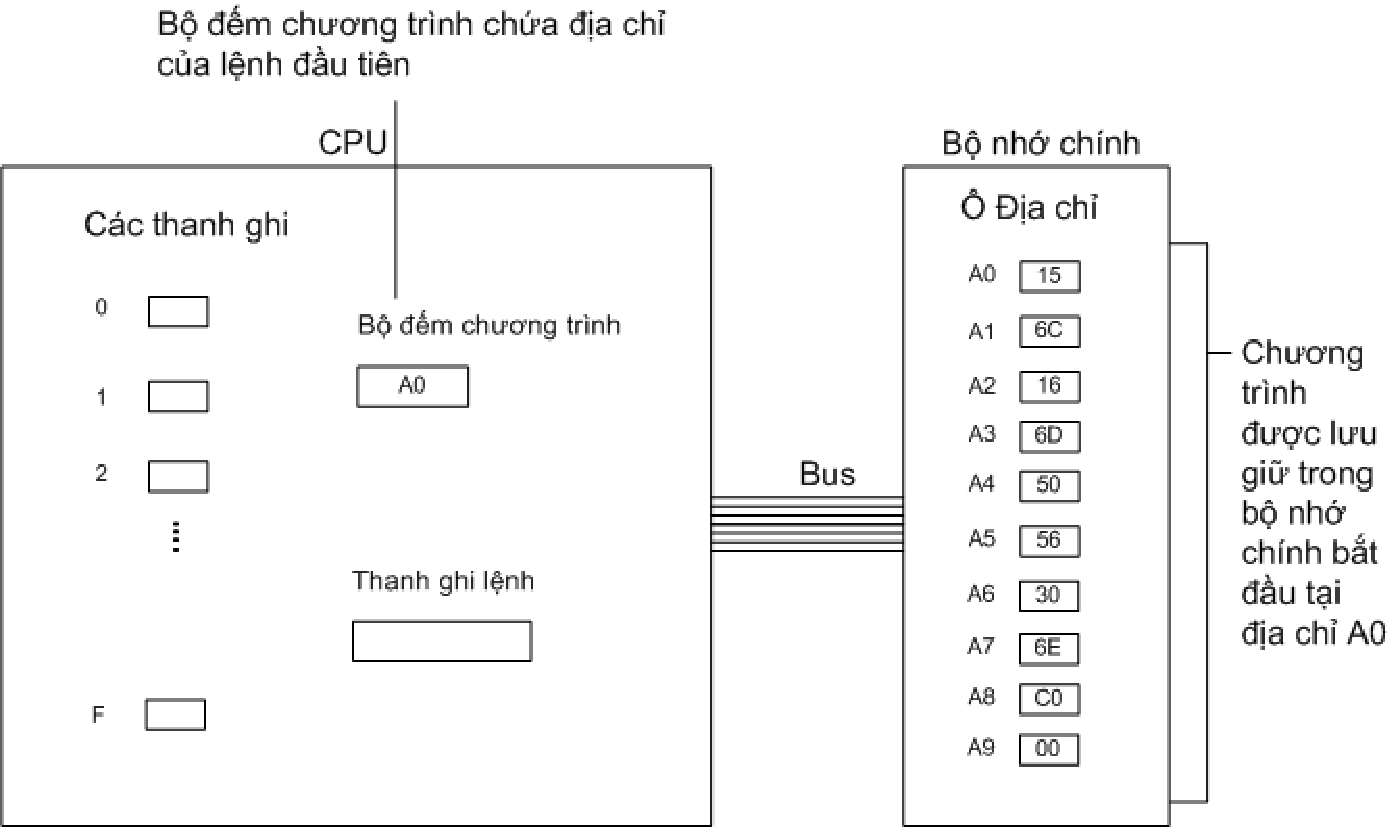
\includegraphics{ch3/fig210.pdf}}
  \caption{Chương trình từ Hình \ref{fig:fig27} được lưu giữ trong bộ nhớ để sẵn sàng thực
    hiện.}
  \label{fig:fig210}
\end{figure}


\begin{figure}
  \centering \subfloat[Lúc bắt đầu của bước nạp, lệnh bắt đầu tại địa chỉ $A0$ được nhận
  từ bộ nhớ và đặt vào thanh ghi lệnh]
  {\scalebox{0.8}{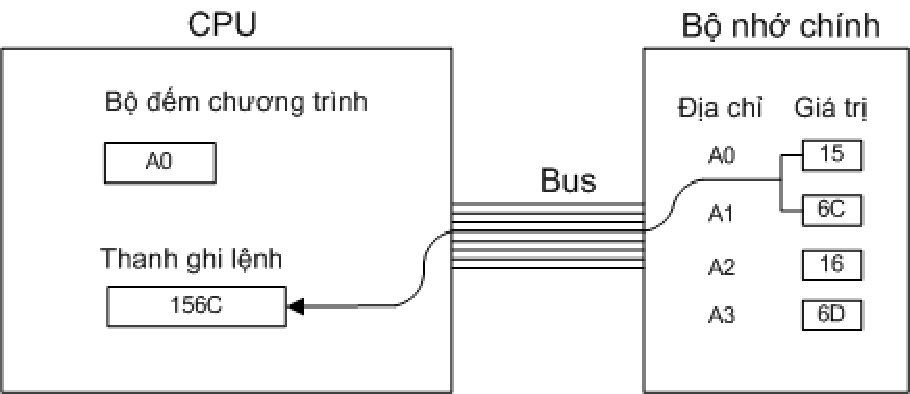
\includegraphics{ch3/fig211a.pdf}} \label{fig:fig211a}}

  \subfloat[Sau đó bộ đếm chương trình tăng lên để trỏ vào lệnh tiếp theo.]
  {\scalebox{0.8}{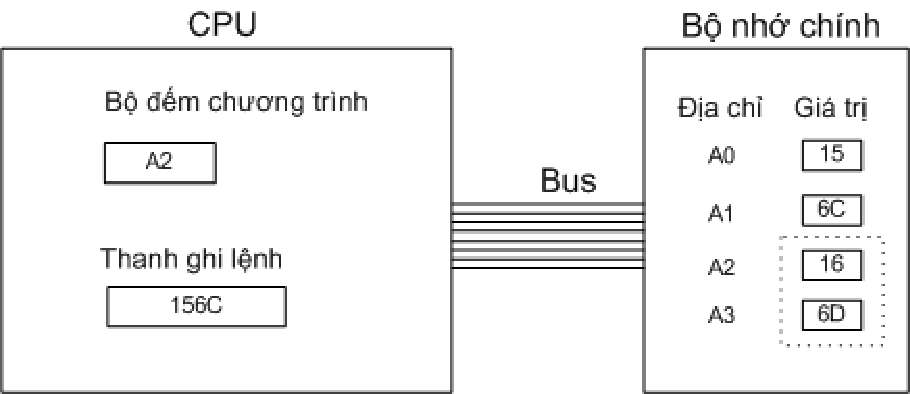
\includegraphics{ch3/fig211b.pdf}} \label{fig:fig211b}}
  \caption{Thực hiện bước nạp của chu kỳ máy.}
\end{figure}


Đơn vị điều khiển bắt đầu bước nạp của chu kỳ máy bằng cách lấy lệnh nằm trong bộ nhớ
chính tại địa chỉ $A0$ và đặt lệnh này ($156C$) trong thanh ghi lệnh (Hình
\ref{fig:fig211a}). Chú ý rằng, một lệnh trong máy của ta có độ dài $16$ bít (bằng $2$
byte). Bởi vậy nó sẽ chiếm hai ô nhớ $A0$ và $A1$ trong bộ nhớ. Đơn vị điều khiển được
thiết kế để đặt nội dung cả hai ô nhớ này vào thanh ghi lệnh (độ dài $16$ bít).  Nó tăng
bộ đếm chương trình lên hai giá trị để trỏ tới địa chỉ của lệnh tiếp theo (Hình
\ref{fig:fig211b}). Vậy, ở cuối bước nạp của chu kỳ máy đầu tiên, bộ đếm chương trình và
thanh ghi lệnh chứa dữ liệu sau đây:

\begin{itemize}
\item[] Bộ đếm chương trình: $A2$

\item[] Thanh ghi lệnh: $156C$
\end{itemize}

Sau đó, đơn vị điều khiển phân tích lệnh trong thanh ghi lệnh và kết luận rằng đây là lệnh
``nạp thanh ghi $5$ bằng nội dung của ô nhớ tại địa chỉ $6C$''.  Việc nạp được thực hiện
trong bước thực hiện của chu kỳ máy. Đơn vị điều khiển lại bắt đầu chu kỳ tiếp theo.

Chu kỳ này bắt đầu với việc nạp lệnh $166D$ từ hai ô nhớ bắt đầu tại địa chỉ $A2$. Đơn vị
điều khiển đặt lệnh này vào thanh ghi lệnh và tăng bộ đếm chương trình lên $A4$. Bây giờ
đơn vị điều khiển giải mã lệnh $166D$ và xác định rằng phải nạp thanh ghi $6$ với nội dung
của ô nhớ tại địa chỉ $6D$. Thanh ghi $6$ được nạp trong bước thực hiện của chu kỳ máy.

Bởi vì bộ đếm chương trình bây giờ chứa $A4$, đơn vị điều khiển đọc lệnh tiếp theo tại địa
chỉ này. Kết quả là $5056$ được đặt trong thanh ghi lệnh, và bộ đếm chương trình được tăng
lên thành $A6$. Đơn vị điều khiển bây giờ giải mã nội dung thanh ghi lệnh và thực hiện nó
bằng cách kích hoạt mạch cộng số bù hai với đầu vào là các thanh ghi $5$ và~$6$.

Trong bước thực hiện này, ALU thực hiện phép cộng và đặt kết quả vào thanh ghi~$0$ (theo
yêu cầu của đơn vị điều khiển), và thông báo với đơn vị điều khiển rằng nó đã kết
thúc. Đơn vị điều khiển sau đó bắt đầu chu kỳ máy khác. Một lần nữa, với sự trợ giúp của
bộ đếm chương trình, nó nạp lệnh tiếp theo ($306E$) từ hai ô nhớ bắt đầu tại địa chỉ $A6$
và tăng bộ đếm chương trình thành $A8$. Lệnh này được giải mã và thực hiện. Tại điểm này,
giá trị tổng được đặt vào ô nhớ tại vị trí $6E$.

Lệnh tiếp theo được nạp bắt đầu tại địa chỉ $A8$, và bây giờ bộ đếm chương trình được tăng
thành $AA$. Nội dung của thanh ghi lệnh là $C000$ và được giải mã là lệnh dừng chương
trình. Kết quả là, máy dừng tại bước thực hiện của chu kỳ máy, và hoàn tất việc chạy
chương trình.

Tóm lại, quá trình mà máy thực hiện lệnh cũng giống như ta đã làm để theo dõi chi
tiết từng lệnh. Nếu ta giữ vị trí bằng cách đánh dấu lệnh thì máy tính sử dụng bộ
đếm chương trình. Sau khi xác định lệnh nào tiếp theo sẽ được thực hiện, ta có thể
đọc lệnh xem ý nghĩa của nó là gì. Điều đó có nghĩa rằng ta đã thực hiện được nhiệm
vụ yêu cầu và quay trở lại danh sách để thực hiện lệnh tiếp theo giống như máy thực hiện
lệnh trong thanh ghi và quay trở lại với quá trình nạp tiếp theo.

\subsection*{Chương trình hay dữ liệu}
Nhiều chương trình có thể được lưu trữ đồng thời trong bộ nhớ chính của máy tính, miễn là
chúng ở những vị trí khác nhau. Việc xác định chương trình nào sẽ được chạy đơn thuần chỉ
là việc đặt một giá trị thích hợp cho bộ đếm chương trình.

Tuy nhiên, ta cũng phải để ý rằng, dữ liệu cũng được chứa trong bộ nhớ chính và được
mã hóa dưới dạng các dãy $0$ và $1$, máy tính không thể biết được đâu là dữ liệu và đâu là
chương trình. Nếu bộ đếm chương trình được trỏ đến một vùng dữ liệu thay vì vùng cho
chương trình, máy tính sẽ đọc các bít dữ liệu như các lệnh và thực hiện chúng. Kết quả
chạy chương trình lúc đó phụ thuộc vào dữ liệu đọc được và không thể dự đoán trước được nó
sẽ làm gì.

Ta cũng không nên kết luận rằng việc để chương trình và dữ liệu nằm chung trong bộ nhớ
chính là ý tưởng tồi. Trên thực tế, điều này rất có ích. Nó cho phép một chương trình thao
tác một chương trình khác (hoặc thậm chí với bản thân nó) giống như nó là dữ liệu. Hãy
tưởng tượng, ví dụ chương trình có khả năng học bằng cách tự thay đổi bản thân nó để phản
hồi lại các tương tác với môi trường bên ngoài. Hoặc thậm chí có tồn lại một loại chương
trình có thể viết và thực hiện một chương trình khác để giải quyết vấn đề cho trước.

\subsection*{Câu Hỏi \& Bài Tập}
\begin{enumerate}
\item Giả sử rằng các ô nhớ tại địa chỉ từ $00$ tới $05$ trong máy mô tả bởi Phụ lục
  \ref{phuluc1} chứa dãy bít (dưới dạng hexa) được cho trong bảng sau:

\begin{tabular}{cc}
  Địa chỉ & Nội dung \\
  $00$    & $14$     \\
  $01$    & $02$     \\
  $02$    & $34$     \\
  $03$    & $17$     \\
  $04$    & $C0$     \\
  $05$     & $00$
\end{tabular}

Nếu ta bắt đầu cho máy chạy với bộ đếm chương trình chưa giá trị $00$, vậy khi máy
dừng thì ô nhớ tại địa chỉ $17$ (ở dạng hexa) sẽ chứa giá trị bao nhiêu?

\item Giả sử rằng các ô nhớ từ $B0$ tới $B8$ trong máy mô tả ở Phụ lục \ref{phuluc1} chứa
  dãy bít (dưới dạng hexa) được cho bởi bảng sau:

\begin{tabular}{cc}
  Địa chỉ & Nội dung \\
  $B0$    & $13$     \\
  $B1$    & $B8$     \\
  $B2$    & $A3$     \\
  $B3$    & $02$     \\
  $B4$    & $33$     \\
  $B5$     & $B8$ \\
  $B6$    & $C0$     \\
  $B7$    & $00$     \\
  $B8$     & $0F$ 
\end{tabular}
\begin{enumerate}
\item Nếu chương trình bắt đầu tại địa chỉ $B0$, nội dung (tính theo bít) của thanh ghi số
  $3$ sau khi lệnh đầu tiên được thực hiện sẽ là bao nhiêu?

\item Nội dung của ô nhớ tại địa chỉ $B8$ là bao nhiêu sau khi lệnh kết thúc chương trình
  được thực hiện?
\end{enumerate}

\item \label{ex:233} Giả sử rằng các ô nhớ từ $A4$ tới $B1$ trong máy mô tả ở Phụ lục
  \ref{phuluc1} chứa dãy bít (dưới dạng hexa) được cho bởi bảng sau:
 
\begin{tabular}{cc}
  Địa chỉ & Nội dung \\
  $A4$    & $20$     \\
  $A5$    & $00$     \\
  $A6$    & $21$     \\
  $A7$    & $03$     \\
  $A8$    & $22$     \\
  $A9$     & $01$ \\
  $AA$    & $B1$     \\
  $AB$    & $B0$     \\
  $AC$     & $50$ \\
  $AD$    & $02$     \\
  $AE$     & $B0$ \\
  $AF$    & $AA$     \\
  $B0$    & $C0$     \\
  $B1$     & $00$ 
\end{tabular}

Hãy trả lời các câu hỏi dưới đây với giả sử rằng máy bắt đầu với bộ đếm chương trình chứa
giá trị $A4$.

\begin{enumerate}
\item Giá trị của thanh ghi $0$ bằng bao nhiêu sau khi lệnh tại địa chỉ $AA$ được thực
  hiện lần đầu tiên?

\item Giá trị của thanh ghi $0$ bằng bao nhiêu khi lệnh tại địa chỉ $AA$ được thực hiện
  lần thứ hai ?

\item Lệnh tại địa chỉ $AA$ sẽ được thực hiện bao nhiêu lần trước khi máy dừng?
\end{enumerate}

\item \label{ex:234} Giả sử rằng các ô nhớ từ $F0$ tới $F9$ trong máy mô tả ở Phụ lục
  \ref{phuluc1} chứa dãy bít (dưới dạng hexa) được cho bởi bảng sau:
 
  \begin{tabular}{cc}
    Địa chỉ & Nội dung \\
    $F0$    & $20$     \\ 
    $F1$    & $C0$     \\
    $F2$    & $31$     \\
    $F3$    & $F8$     \\
    $F4$    & $20$     \\
    $F5$     & $00$ \\
    $F6$    & $30$     \\
    $F7$    & $F9$     \\
    $F8$     & $FF$ \\
    $F9$    & $FF$     \\
  \end{tabular}

  Nếu ta cho máy bắt đầu với bộ đếm chương trình chứa $F0$, máy thực hiện nhiệm vụ
  gì khi nó đi tới lệnh tại địa chỉ $F8$?
\end{enumerate}

\section{Các lệnh số học và logic}
\label{sec:2.4}
Như đã chỉ ra ở phần trước, nhóm lệnh số học và logic bao gồm các lệnh thực hiện các phép
toán số học, logic và các phép toán dịch. Trong phần này, ta sẽ xem chi tiết các
phép toán này.

\subsection*{Các Phép Toán Logic}
Ta đã xem xét các phép toán logic $\AND$, $\OR$, $\XOR$ (tuyển loại) trong Chương
\ref{chap:1}, như các phép toán hai ngôi, có hai đầu vào và một đầu ra đều một bít. Các
phép toán này có thể mở rộng cho đầu vào, đầu ra là các dãy bít bằng cách áp dụng các phép
toán cơ bản cho các từng bít tương ứng trong dãy. Ví dụ, kết quả của việc $\AND$ hai dãy
bít $10011010$ và $11001001$ cho kết quả là
\begin{flushleft}
  \begin{tabular}{ll}
    & $10011010$ \\
    $\AND$ & $11001001$\\
    \hline
    &10001000
  \end{tabular}
\end{flushleft}
bằng việc đơn thuần áp dụng phép toán $\AND$ cho từng cặp bít tương ứng ở các cột. Cũng
tương tự, cho các phép toán $\OR$ và $\XOR$
\begin{flushleft}
  \begin{tabular}{ll}
    & $10011010$ \\
    $\OR$ & $11001001$\\
    \hline
    &11011011
  \end{tabular}
  \qquad \qquad \qquad
  \begin{tabular}{ll}
    & $10011010$ \\
    $\XOR$ & $11001001$\\
    \hline
    &01010011
  \end{tabular}
\end{flushleft}

Một trong những ứng dụng chính của phép toán $\AND$ là ẩn một phần của dãy bít không làm
ta quan tâm. Ta xem xét, ví dụ, chuyện gì xảy ra nếu byte $00001111$ là toán hạng
đầu tiên của phép toán $\AND$. Không cần biết về nội dung của toán hạng thứ hai, ta
vẫn có thể kết luận rằng bốn bít trái nhất của dãy bít kết quả sẽ là $0$. Hơn nữa, bốn bít
phía phải của kết quả sẽ sao chép phần tương ứng của toán hạng thứ hai, như được chỉ ra
trong ví dụ dưới đây:
\begin{flushleft}
  \begin{tabular}{ll}
    & $00001111$ \\
    $\AND$ & $10101010$\\
    \hline
    &$00001010$
  \end{tabular}
\end{flushleft}

Cách sử dụng phép toán $\AND$ trong trường hợp này là một ví dụ của xử lý \textbf{mặt
  nạ}. Ở đây, một phép toán, được gọi là \textbf{mặt nạ}, xác định phần của toán hạng khác
sẽ ảnh hưởng đến kết quả. Trong trường hợp của phép toán $\AND$ ở trên, mặt nạ sẽ cho kết
quả là bản sao của một phép toán, với các bít $0$ sẽ thay thế vào các vị chí không cần sao
chép.

Như vậy, đây là một phép toán có ích khi thao tác với \textbf{ánh xạ bít}, là một xâu bít
trong đó mỗi bít dùng để biểu diễn sự có mặt hay vắng mặt của một đối tượng. Một ví dụ là
các ánh xạ bít trong các ứng dụng xử lý ảnh, ở đó mỗi bít được gắn với một điểm ảnh.

Vậy thì, giả sử rằng một ô nhớ tám bít (một byte) đang được sử dụng như một ánh xạ bít, và
ta muốn biết đối tượng gắn với bít thứ ba từ cao xuống thấp có mặt hay không; chúng
ta chỉ cần $\AND$ byte này với mặt nạ $00100000$, nó sẽ cho kết quả là một byte gồm toàn
bít $0$ nếu và chỉ nếu bít thứ ba từ cao xuống thấp có giá trị là $0$. Hơn nữa, nếu ta
muốn đặt bít thứ ba từ cao xuống thấp bằng $0$ mà không muốn tác động tới các bít khác,
vậy thì ta có thể $\AND$ ánh xạ bít với mặt nạ $11011111$ và lưu trữ lại kết quả vào
ánh xạ bít ban đầu.

Trong khi phép toán $\AND$ có thể được sử dụng để sao chép một phần dãy bít bằng cách đặt
các bít $0$ vào phần không cần sao chép, thì phép toán $\OR$ có thể sử dụng để sao chép
một phần của dãy bít bằng cách đặt các giá trị $1$ vào phần không cần sao chép. Để làm
điều này, một lần nữa ta lại sử dụng một mặt nạ, nhưng lần này ta chỉ ra những
vị trí bít được sao chép với các bít $0$, còn các bít $1$ chỉ ra các phần không sao
chép. Ví dụ, khi ta $\OR$ một byte với $11110000$ sẽ cho kết quả là $1111$ trong bốn bít
cao, còn bốn bít thấp là bản sao bốn bít thấp của toán hạng kia, như dưới đây:
\begin{flushleft}
  \begin{tabular}{ll}
    & $11110000$ \\
    $\OR$ & $10101010$\\
    \hline
    &$11111010$
  \end{tabular}
\end{flushleft}
Kết quả là, trong khi mặt nạ $11011111$ có thể sử dụng với phép toán $\AND$ để đặt giá trị
$0$ vào bít thứ ba từ cao xuống thấp, thì mặt nạ $00100000$ có thể được sử dụng với phép
toán $\OR$ để đặt giá trị $1$ vào vị trí này.

Một trong những ứng dụng chính của phép toán $\XOR$ là để tính phần bù của một dãy
bít. Nếu $\XOR$ một byte tuỳ ý với mặt nạ gồm tám số $1$, thì ta sẽ được phần bù của byte
này. Ví dụ, để ý quan hệ giữa toán hạng thứ hai và kết quả trong ví dụ dưới đây:
\begin{flushleft}
  \begin{tabular}{ll}
    & $11111111$ \\
    $\XOR$ & $10101010$\\
    \hline
    &$01010101$
  \end{tabular}
\end{flushleft}

Trong ngôn ngữ máy mô tả trong Phụ lục \ref{phuluc1}, các op-code $7,8$ và $9$ được sử
dụng cho các phép toán logic $\AND$, $\OR$, và $\XOR$, tương ứng. Các phép toán này yêu
cầu đầu vào là hai thanh ghi và cho ra kết quả vào một thanh ghi. Ví dụ, lệnh $7ABC$ thực
hiện $\OR$ nội dung của thanh ghi $B$ với thanh ghi $C$ và đặt kết quả vào thanh ghi $A$.

\subsection*{Các phép toán quay  và dịch}
Các phép toán trong nhóm các phép toán quay và dịch cho phép dịch chuyển các bít bên trong
một thanh ghi. Các phép toán này được phân loại theo hướng dịch chuyển (trái hoặc phải)
hoặc là xử lý quay vòng. Ta có thể xây dựng nhiều phép toán bằng cách kết hợp các khả năng
đó lại. Ta sẽ lướt nhanh các ý tưởng liên quan.

Xét một thanh ghi tám bít (một byte), nếu ta dịch nội dung của nó sang phải một bít, ta
tưởng tượng rằng bít phải nhất sẽ bị rơi ra ngoài và một lỗ trống sẽ xuất hiện ở phía trái
nhất. Nếu bít bị rơi ra ngoài và lỗ trống là khác nhau sẽ cho ta nhiều cách dịch khác
nhau. Một cách dịch là đặt bít rơi ra ngoài phía bên phải vào lỗ trống phía bên trái; kết
quả ta có \textbf{dịch vòng}, cũng còn được gọi là \textbf{quay}. Nếu ta thực hiện phép
toán quay tám lần trên một byte, thì ta đạt được chính xâu bít ban đầu.

Một kỹ thuật khác là loại bỏ bít rơi ra và luôn đặt vào lỗ trống giá trị $0$. Thuật ngữ
\textbf{dịch logic} thường được dùng cho phép toán này. Nói chung, việc dịch trái một số
nhị phân tương đương với việc nhân nó với hai, cũng tương tự như dịch trái một số thập
phân tương đương với việc nhân nó với mười. Hơn nữa, phép chia cho hai cũng có thể được
thực hiện bằng cách dịch phải. Với ý nghĩa này, trong cả hai phép dịch, ta đều phải cẩn
thận bảo toàn bít dấu trong một số hệ thống ký hiệu (ví dụ với biểu diễn bù hai). Bởi vậy,
ta thường thấy một số kiểu dịch phải luôn bảo toàn giá trị gốc của lỗ trống để giữ bít
dấu. Các phép dịch mà bít dấu không thay đổi đôi khi được gọi là phép \textbf{dịch số
  học}.

Mặc dù các phép toán dịch và quay phong phú như vậy, ngôn ngữ máy mô tả trong phần Phụ lục
\ref{phuluc1} chỉ có phép toán quay phải, với op-code là $A$. Trong trường hợp này số hexa
đầu tiên trong trường toán hạng xác định thanh ghi được quay, phần còn lại xác định số bít
cần quay. Bởi vậy lệnh $A501$ có nghĩa rằng ``Quay nội dung thanh ghi $5$ sang phải $1$
bít''.  Cụ thể, nếu thanh ghi $5$ ban đầu có nội dung là $65$ (hexa), vậy thì nó sẽ
chứa~$B2$ sau khi lệnh được thực hiện (Hình~\ref{fig:fig212}).  Các phép dịch và quay khác
có thể tạo ra bằng cách tổ hợp các lệnh trong ngôn ngữ máy của Phụ lục \ref{phuluc1}. Ví
dụ, với một thanh ghi $8$ bít, việc dịch phải ba bít đồng nhất với việc dịch trái năm bít.

\begin{figure}[tbh]
  \centering {\scalebox{0.7}{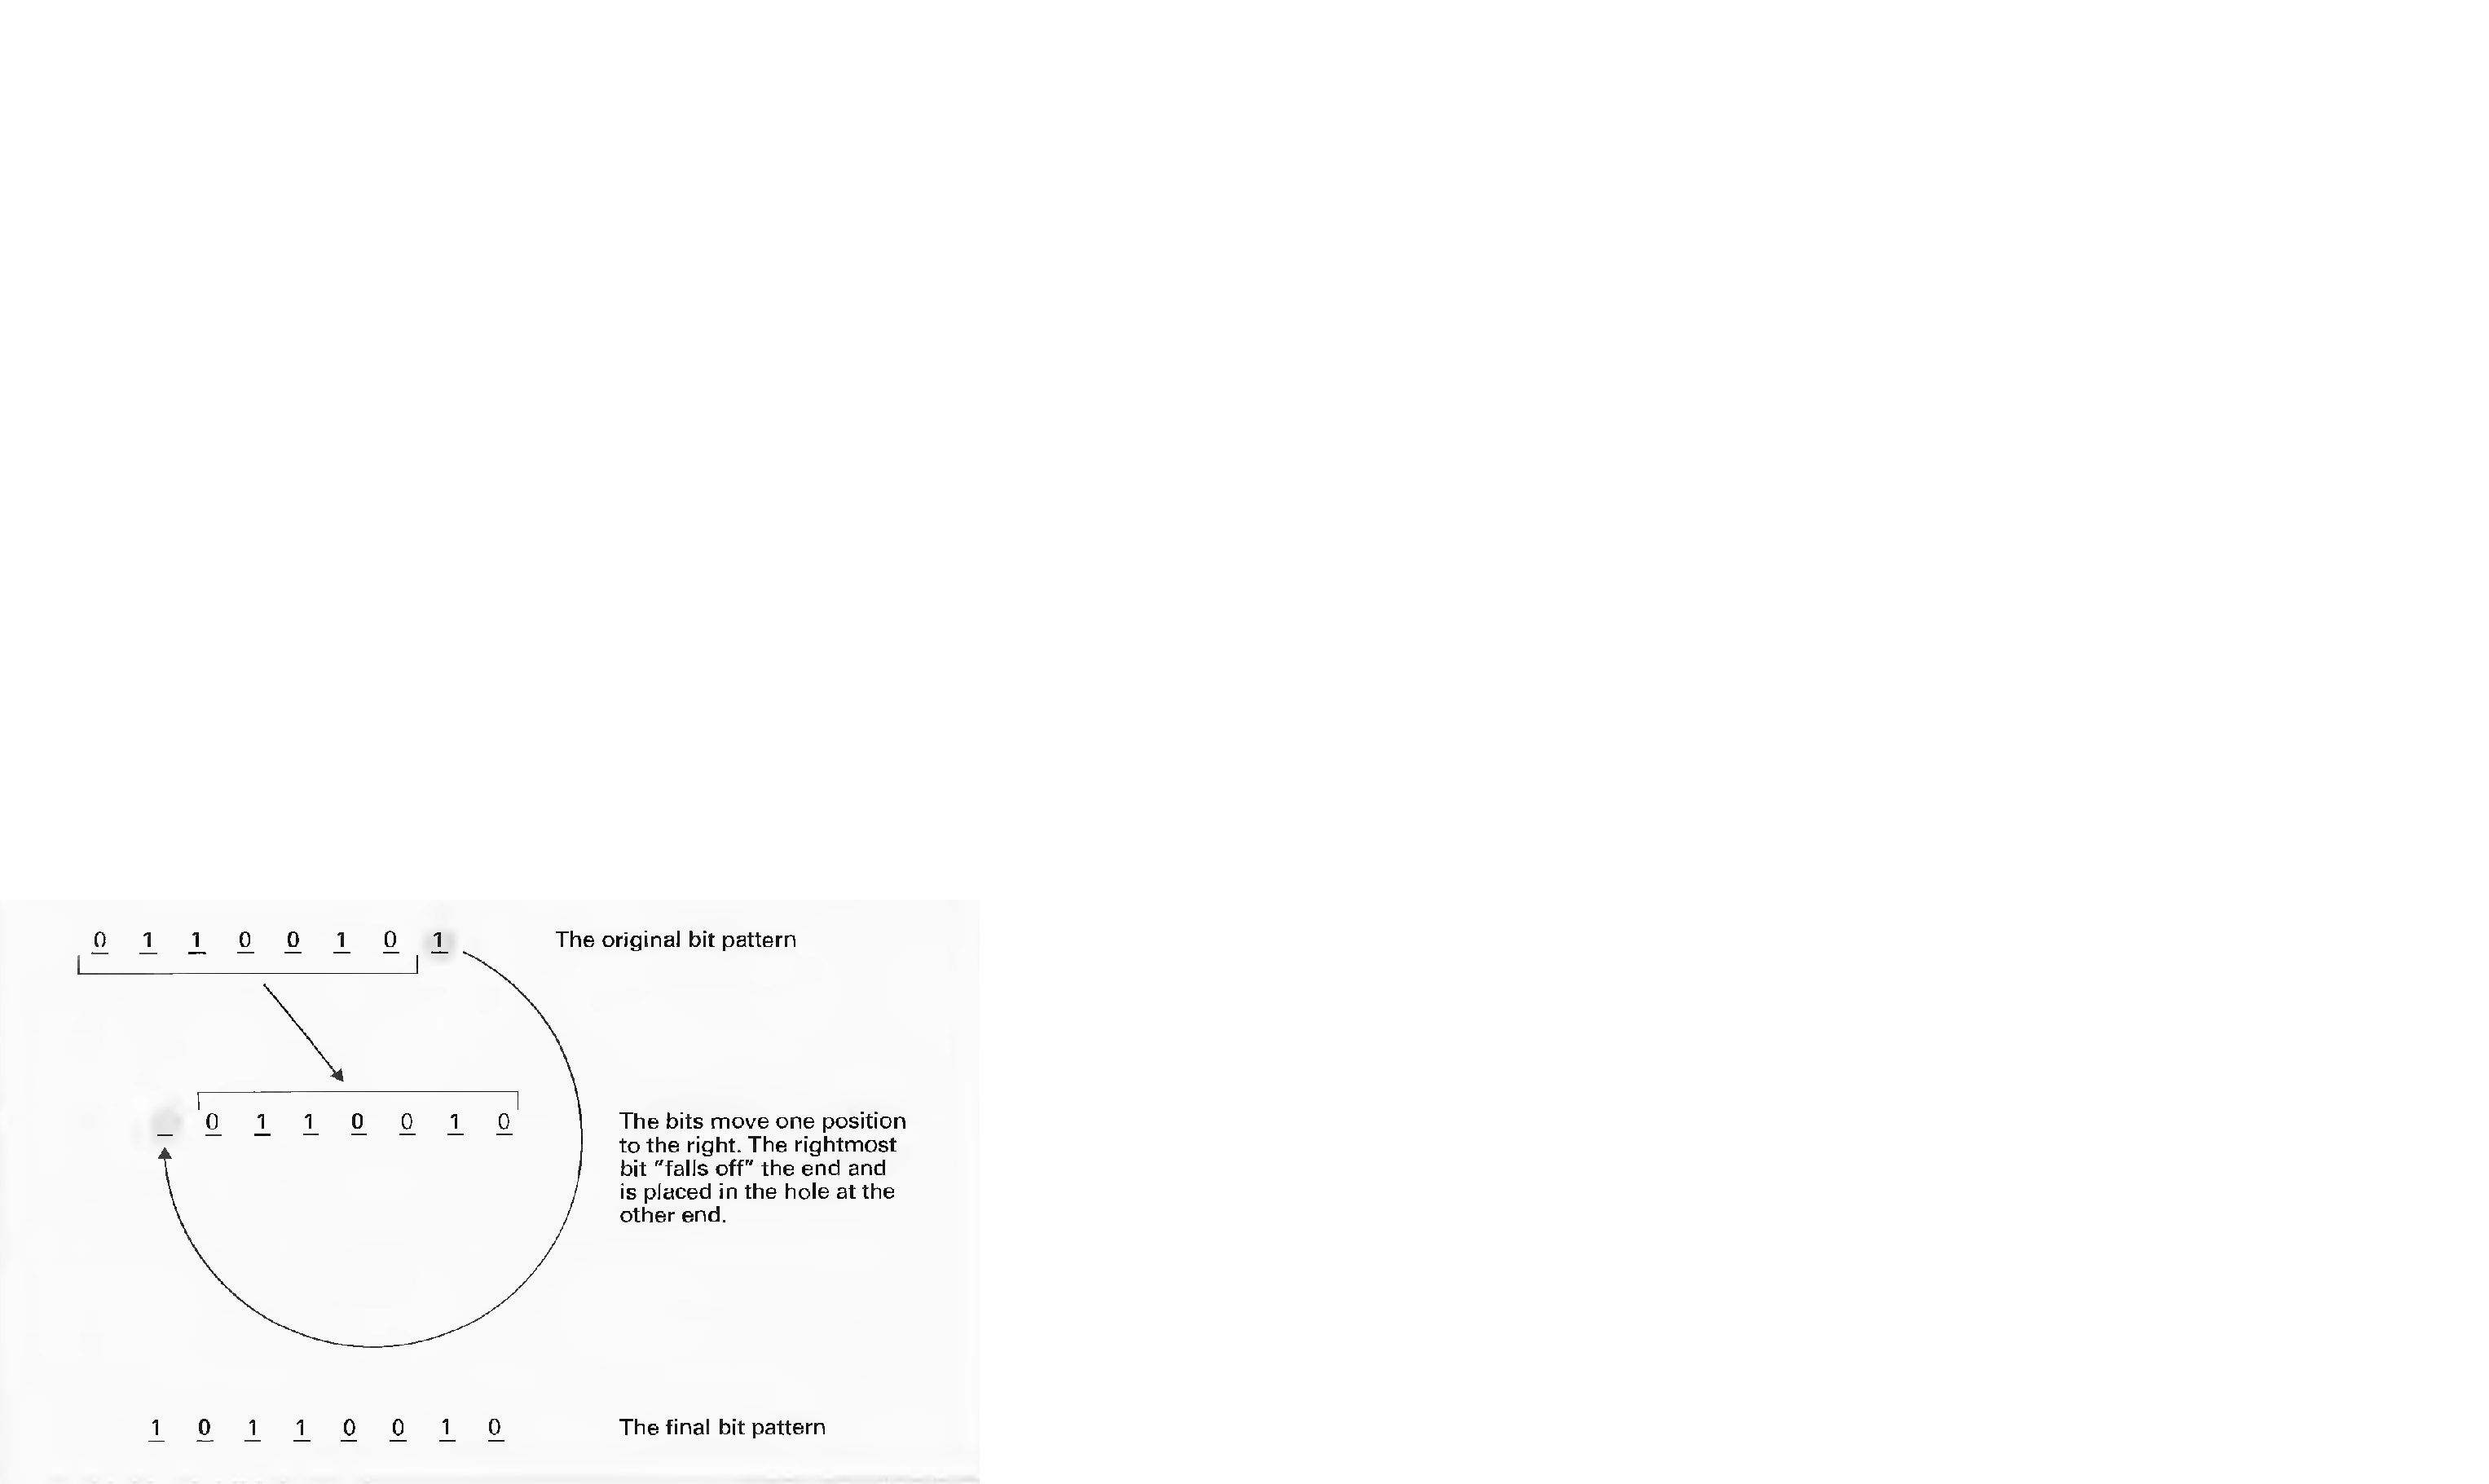
\includegraphics{ch3/fig212.pdf}} }
  \caption{Quay xâu bít $65$ ở dạng hexa sang phải một bít.}
  \label{fig:fig212}
\end{figure}

\subsection*{Các phép toán số học}

Mặc dù ta đã thảo luận về các phép toán số học cộng, trừ, nhân, và chia; nhưng ta cần chú
ý rằng giữa chúng có một vài liên hệ không rõ ràng lắm. Đầu tiên, ta đã thấy rằng phép trừ
có thể được thực hiện nhờ phép cộng và phép lấy phần bù. Hơn nữa, phép nhân chỉ đơn thuần
là lặp lại của phép cộng; và phép chia đơn thuần là lặp lại của phép trừ (ví dụ, sáu chia
cho hai bằng ba bởi vì sáu trừ cho hai chỉ được nhiều nhất là ba lần). Vì lý do này, một
vài CPU nhỏ được thiết kế chỉ có lệnh cộng hoặc chỉ có lệnh cộng hoặc trừ.

Ta để ý rằng có một vài điểm khác biệt tồn tại giữa các hệ thống số (điều này cũng
liên quan đến hai phép toán cộng có sẵn trong máy ở Phụ lục \ref{phuluc1}). Ví dụ, nếu giá
trị được cộng biểu diễn dưới dạng bù hai, quá trình cộng sẽ phải thực hiện cộng từng bít
tương ứng theo cột. Tuy nhiên, nếu các toán hạng được lưu trữ theo kiểu dấu chấm động, quá
trình cộng phải thực hiện đọc phần định trị của mỗi toán hạng, dịch chúng sang phải hoặc
trái theo phần số mũ, kiểm tra bít dấu, thực hiện phép cộng, và dịch kết quả ra theo ký
hiệu dấu phảy động. Bởi vậy, mặc dù cả hai đều là phép cộng, hoạt động của máy để thực
hiện chúng là khác nhau.

\subsection*{Câu Hỏi \& Bài Tập}
\begin{enumerate}
\item Thực hiện các phép toán sau.

  \begin{inparaenum}[a. ]
  \item \begin{tabular}{m{1cm}l}
      & $01001011$\\
      $\AND$ & $10101011$\\
      \hline
    \end{tabular} \quad
  \item \begin{tabular}{m{1cm}l}
      & $10000011$\\
      $\AND$ & $11101100$\\
      \hline
    \end{tabular} \quad
  \item \begin{tabular}{m{1cm}l}
      & $11111111$\\
      $\AND$ & $00101101$\\
      \hline
    \end{tabular}

    \bigskip

  \item \begin{tabular}{m{1cm}l}
      & $01001011$\\
      $\OR$ & $11101100$\\
      \hline
    \end{tabular} \quad 
  \item \begin{tabular}{m{1cm}l}
      & $10000011$\\
      $\OR$ & $11101100$\\
      \hline
    \end{tabular} \quad 
  \item \begin{tabular}{m{1cm}l}
      & $11111111$\\
      $\OR$ & $00101101$\\
      \hline
    \end{tabular}


    \bigskip

  \item \begin{tabular}{m{1cm}l}
      & $01001011$\\
      $\XOR$ & $11101100$\\
      \hline
    \end{tabular} \quad 
  \item \begin{tabular}{m{1cm}l}
      & $10000011$\\
      $\XOR$ & $11101100$\\
      \hline
    \end{tabular} \quad 
  \item \begin{tabular}{m{1cm}l}
      & $11111111$\\
      $\XOR$ & $00101101$\\
      \hline
    \end{tabular}
  \end{inparaenum}

\bigskip

\item Giả sử rằng bạn muốn cô lập bốn bít giữa của một byte bằng cách đặt các số~$0$ vào
  bốn bít còn lại. Vậy bạn phải sử dụng mặt nạ và phép toán gì để làm điều này?

\item Giả sử rằng bạn muốn tính phần bù của bốn bít giữa của một byte mà không muốn tác
  động vào các bít khác. Vậy bạn phải sử dụng mặt nạ gì và với phép toán gì để làm điều
  này?

\item
  \begin{enumerate}
  \item Giả sử rằng bạn thực hiện $\XOR$ hai bít đầu tiên của một xâu bít và sau đó tiếp
    tục $\XOR$ bít kết quả với bít tiếp theo, lại tiếp tục kết quả với bít tiếp
    theo... cho đến hết xâu. Kết quả cuối cùng có liên quan như thế nào đến số số $1$ xuất
    hiện trong xâu?

  \item Bài toán này có liên quan như thế nào trong việc xác định bít chẵn lẻ khi mã hoá
    thông điệp?

  \end{enumerate}

\item Thông thường, việc sử dụng các phép toán logic là thích hợp hơn so với dùng phép
  toán trên số. Ví dụ, phép toán logic $\AND$ tổ hợp hai bít giống như phép nhân. Phép
  toán logic nào gần giống như phép cộng hai số? phép toán logic bạn chỉ ra đó khác phép
  cộng trong trường hợp nào?

\item Phép toán logic cùng với mặt nạ nào có thể dùng để đổi các mã ASCII từ mã của chữ
  thường thành mã của chữ hoa? và ngược lại, từ chữ hoa thành chữ thường?

\item Kết quả thực hiện việc quay sang phải ba bít trên các xâu bít sau đây là gì?

  \begin{inparaenum}[a. ]
  \item $01101010$ \qquad \qquad \qquad
  \item $00001111$ \qquad \qquad \qquad
  \item $01111111$
  \end{inparaenum}

\item Kết quả của việc quay một bít sang trái trên các byte được biểu diễn bởi các ký hiệu
  hexa dưới đây là gì? Hãy đưa ra kết quả ở dạng hexa.

  \begin{inparaenum}[a. ]
  \item $AB$ \qquad \qquad \qquad
  \item $5C$ \qquad \qquad \qquad
  \item $B7$ \qquad \qquad \qquad
  \item $35$
  \end{inparaenum}


\item Quay một xâu tám bít sang phải ba bít thì tương đương với quay nó sang trái bao
  nhiêu bít?

\item Xâu bít nào biểu diễn tổng của $01101010$ với $11001100$ nếu chúng được biểu diễn
  dưới dạng bù hai? nếu chúng được lưu trữ dưới dạng dấu chấm động như thảo luận ở Chương
  \ref{chap:1}?

\item Sử dụng ngôn ngữ máy ở Phụ lục \ref{phuluc1}, hãy viết chương trình đặt giá trị $1$
  vào bít trái nhất của ô nhớ tại địa chỉ $A7$ mà không thay đổi các bít khác.

\item Sử dụng ngôn ngữ máy ở Phụ lục \ref{phuluc1}, hãy viết chương trình sao chép bốn bít
  giữa từ ô nhớ $E0$ vào bốn bít thấp của ô nhớ tại địa chỉ $E1$ bằng cách đặt các giá trị
  $0$ vào bốn bít cao nhất của ô nhớ tại địa chỉ $E1$.

\end{enumerate}

\section{Giao tiếp với các thiết bị khác}
\label{sec:2.5}
Bộ nhớ chính và CPU là trung tâm của máy tính. Trong phần này, ta sẽ thảo luận làm thế nào
phần trung tâm này, cái mà ta sẽ gọi là máy tính, giao tiếp với các thiết bị ngoại vi như
hệ thống lưu trữ khối, máy in, bàn phím, chuột, màn hình, camera số, và thậm chí với máy
tính khác.

\subsection*{Vai Trò của Bộ Điều Khiển}

Việc giao tiếp giữa máy tính và các thiết bị khác thông thường được thực hiện thông qua
một bộ phận trung gian gọi là \textbf{bộ điều khiển}. Trong trường hợp máy tính cá nhân,
một bộ điều khiển có thể bao gồm hệ thống mạch điện cắm vào bảng mạch chính của máy tính
hoặc, cho tính mềm dẻo, nó có thể có dạng một bảng mạch điện cắm vào khe cắm trên bảng
mạch chính. Trong cả hai trường hợp, bộ điều khiển nối bằng cáp bên trong máy tính tới các
thiết bị ngoại vi hoặc có thể tới bộ kết nối, gọi là \textbf{cổng} (port), nằm phía sau
máy tính ở đó các thiết bị bên ngoài có thể gắn với nó. Các bộ điều khiển này đôi khi bản
thân nó cũng là một máy tính nhỏ, cũng có bộ nhớ của mạch và CPU đơn giản thực hiện chương
trình điều khiển.

Bộ điều khiển dịch các thộng điệp và dữ liệu đến/đi thành dạng tương thích giữa đặc trưng
bên trong của máy tính và thiết bị ngoại vi gắn với nó. Ban đầu, mỗi bộ điều khiển được
thiết kế cho một kiểu thiết bị đặc biệt. Bởi vậy, mua thêm một thiết bị ngoại vi mới cũng
phải mua thêm bộ điều khiển mới.

Tuy nhiên gần đây, một vài giải pháp đã được đưa ra trong lĩnh vực máy tính cá nhân để
chuẩn hoá, như là \textbf{Universal Serial Bus (USB)} và \textbf{FireWire}. Theo cách này,
một bộ điều khiển có thể điều khiển rất nhiều thiết bị. Ví dụ, một bộ điều khiển USB có
thể được sử dụng để giao tiếp giữa máy tính và một tập các thiết bị tương thích USB. Danh
sách các thiết bị này trên thị trường hiện nay bao gồm chuột, máy in, máy scan, thiết bị
lưu trữ khối, và camera số.

Mỗi bộ điều khiển giao tiếp với máy tính cũng sử dụng cùng một bus kết nối mà CPU của máy
tính và bộ nhớ chính sử dụng để giao tiếp với nhau (Hình~\ref{fig:fig213}). Nó có thể theo
dõi tín hiệu đang được gửi giữa CPU và bộ nhớ cũng như đặt tín hiệu của nó vào trong bus.

\begin{figure}
  \centering \scalebox{0.5}{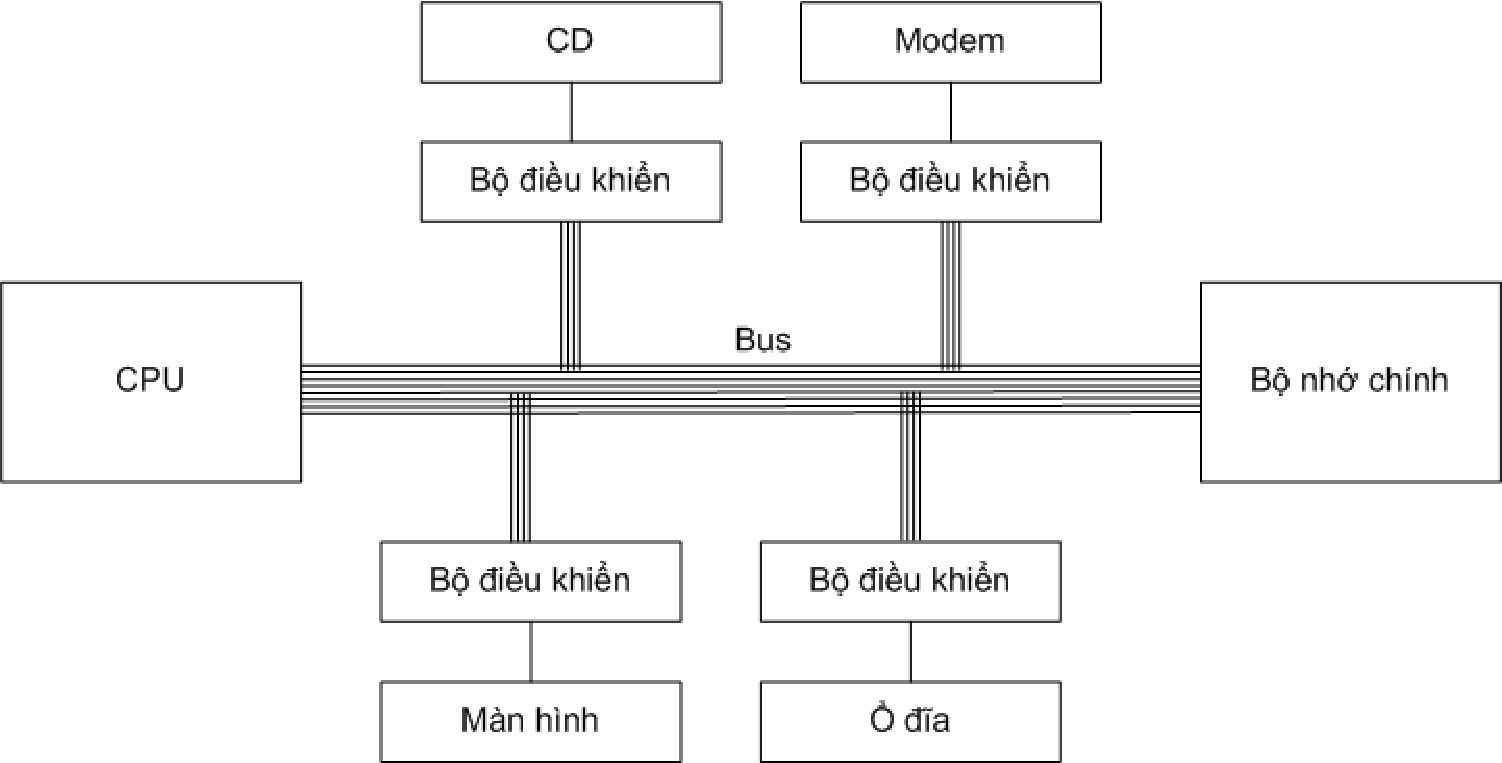
\includegraphics{ch3/fig213.pdf}}
  \caption{Bộ điều khiển gắn với một Bus của máy.}
  \label{fig:fig213}
\end{figure}

Với cách bố trí này, CPU có thể giao tiếp với các bộ điều khiển được gắn với bus giống như
nó giao tiếp với bộ nhớ chính. Để gửi một dãy bít tới bộ điều khiển, dãy bít đầu tiên phải
nằm trong thanh ghi đa năng. Và một lệnh tương tự như lệnh STORE sẽ được thực hiện bởi CPU
để ``lưu trữ'' dữ liệu vào bộ điều khiển. Để nhận một dãy bít từ bộ điều khiển, một lệnh
tương tự lệnh~LOAD sẽ được sử dụng.

Có một vài kiểu máy tính được thiết kế để chuyển dữ liệu từ/tới bộ điều khiển dùng cùng
op-code LOAD và STORE, là các lệnh giao tiếp với bộ nhớ chính. Trong các trường hợp này,
bộ xử lý được thiết kế để đáp ứng lại các ô nhớ tại các chỉ xác định gán cho các bộ điều
khiển. Trong khi đó bộ nhớ chính được thiết kế để bỏ qua các vị trí này. Bởi vậy, khi CPU
gửi thông điệp tới bus để lưu trữ một dãy bít tại các ô nhớ được gán cho bộ điều khiển,
dãy bít này thực sự được ``lưu trữ'' trong bộ điều khiển thay vì trong bộ nhớ. Tương tự,
nếu CPU cố gắng đọc dữ liệu từ một vị trí bộ nhớ như vậy bằng lệnh~LOAD, nó sẽ nhận được
dãy bít từ đơn vị điều khiển thay vì từ bộ nhớ. Cách giao tiếp này được gọi là \textbf{ánh
  xạ bộ nhớ I/O} bởi vì các thiết bị vào/ra của máy tính được ánh xạ vào trong các vùng
nhớ khác nhau (Hình~\ref{fig:fig214}).

\begin{figure}
  \centering \scalebox{0.5}{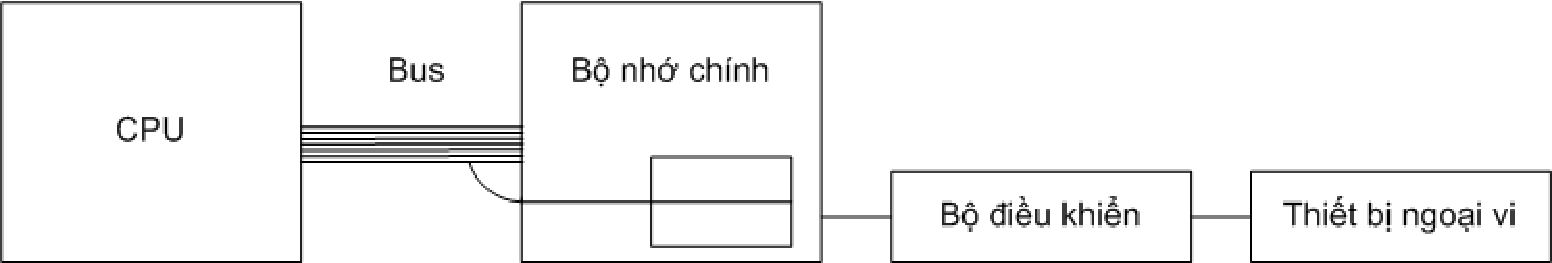
\includegraphics{ch3/fig214.pdf}}
  \caption{Biểu diễn khái niệm của ánh xạ bộ nhớ I/O.}
  \label{fig:fig214}
\end{figure}

Một lựa chọn thay thế cho ánh xạ bộ nhớ I/O là đưa ra một op-code đặc biệt ở ngôn ngữ máy
để chuyển trực tiếp tới/từ bộ điều khiển. Các lệnh với các op-code này được gọi là lệnh
I/O. Ví dụ, nếu ngôn ngữ mô tả trong Phụ lục \ref{phuluc1} theo cách tiếp cận này, nó có
thể có một lệnh kiểu như $F5A3$ với ý nghĩa rằng ``STORE nội dung của thanh ghi $5$ vào
trong bộ điều khiển xác định bởi dãy bít $A3$''.

\subsection*{Truy cập bộ nhớ trực tiếp (DMA)}
Bởi vì bộ điều khiển gắn với bus của máy tính, nó có thể thực hiện giao tiếp với bộ nhớ
chính thông qua bus (tính theo nano giây) khi CPU không sử dụng bus. Khả năng truy cập vào
bộ nhớ chính của bộ điều khiển được gọi là \textbf{truy cập bộ nhớ trực tiếp (DMA)}, và đó
là một khả năng đáng giá cho hiệu năng của máy tính. Ví dụ, để lưu trữ dữ liệu lấy từ một
sector của đĩa, CPU có thể gửi yêu cầu (được mã hoá dưới dạng một dãy bít) tới bộ điều
khiển gắn với đĩa yêu cầu đọc sector và đặt dữ liệu vào một vùng nhớ xác định của bộ
nhớ. Trong khi bộ điều khiển thực hiện thao tác đọc và gửi dữ liệu tới bộ nhớ chính qua
DMA thì CPU tiếp tục làm nhiệm vụ khác. Bởi vậy hai hoạt động sẽ được thực hiện đồng
thời. CPU vẫn thực hiện chương trình và bộ điều khiển phụ trách việc chuyển dữ liệu giữa
đĩa và bộ nhớ chính. Bằng cách này, CPU không mất thời gian liên quan đến việc chuyển dữ
liệu vốn rất chậm chạp.

Việc sử dụng DMA cũng có nhiều bất lợi do ảnh hưởng của việc truyền thông phức tạp trên
bus. Các dãy bít được chuyển giữa CPU và bộ nhớ chính, giữa CPU và các bộ điều khiển, giữa
các bộ điều khiển và bộ nhớ chính. Điều phối được tất cả những hoạt động này trên bus là
vấn đề lớn. Thậm chí với một thiết kế tốt, trung tâm của bus có thể trở thành một trở ngại
cho CPU và bộ điều khiển hoàn thành nhiệm vụ. Trở ngại này được biết như \textbf{trở ngại
  von Neumann} bởi vì nó là hệ quả của \textbf{kiến trúc von Neumann}-- CPU nạp các lệnh
của nó từ bộ nhớ vào bus trung tâm.

\subsection*{Phương pháp bắt tay (Hand Shaking)}

Chuyển dữ liệu giữa hai thành phần máy tính hiếm khi chỉ theo một chiều. Thậm chí dù ta
nghĩ rằng máy in chỉ là một thiết bị nhận dữ liệu, trên thực tế nó cũng gửi dữ liệu trở
lại máy tính. Bởi vì một máy tính có thể gửi dữ liệu tới máy in nhanh hơn rất nhiều so với
khả năng máy in có thể in chúng, nên nếu máy tính cứ nhắm mắt gửi dữ liệu, máy in sẽ bị
tụt hậu một cách nhanh chóng, và kết quả là bị mất dữ liệu. Bởi vậy một quá trình như in
dữ liệu liên quan đến hội thoại hai chiều, được biết như \textbf{bắt tay} (handshaking),
trong đó máy tính và thiết bị ngoại vi trao đổi thông tin về trạng thái thiết bị và điều
phối hoạt động của chúng.

Phương pháp bắt tay liên quan đến một \textbf{từ trạng thái} (status word), là một xâu bít
được sinh bởi thiết bị ngoại vi và gửi tới bộ điều khiển. Từ trạng thái là một \textit{ánh
  xạ bít} dùng để phản hồi lại trạng thái của thiết bị. Ví dụ, trong trường hợp của máy
in, giá trị của bít cao nhất của từ trạng thái có thể chỉ ra khi nào máy in hết giấy,
trong khi đó bít tiếp theo chỉ ra khi nào máy in sẵn sàng thêm dữ liệu. Một bít khác có
thể sử dụng để chỉ ra tình trạng kẹt giấy,... Phụ thuộc vào hệ thống, bộ điều khiển có thể
phản hồi thông tin trạng thái của nó hay nó sẵn sàng với CPU. Trong cả hai trường hợp, từ
trạng thái cho ta một cơ chế để điều phối việc giao tiếp với thiết bị ngoại vi.

\subsection*{Các phương tiện truyền thông  phổ biến}
Việc truyền thông giữa thiết bị tính toán được thực hiện trên hai kiểu truyền: song song
và tuần tự. Các thuật ngữ này chỉ ra cách mà tín hiệu được truyền. Trong trường hợp
\textbf{truyền song song}, nhiều tín hiệu được truyền cùng lúc, mỗi tín hiệu trên một
``đường'' riêng. Kỹ thuật kiểu này cho phép truyền dữ liệu nhanh chóng nhưng yêu cầu đường
truyền phức tạp. Một ví dụ kiểu này là bus bên trong máy tính, nó có nhiều dây cho phép
truyền cả khối dữ liệu và cả tín hiệu khác đồng thời. Hơn nữa, hầu hết các PC đều cho phép
ít nhất một ``cổng song song'' để qua đó dữ liệu có thể truyền cùng lúc tám bít tới/từ máy
tính.

Ngược lại, \textbf{truyền tuần tự} dựa trên việc truyền tín hiệu lần lượt, tín hiệu này
rồi mới đến tín hiệu khác, trên một đường truyền đơn. Bởi vậy, truyền tuần tự yêu cầu
đường dữ liệu đơn giản hơn so với truyền song song, đó là một lý do làm nó trở nên phổ
biến. Ví dụ về truyền tuần tự là USB và FireWire, cả hai đều liên quan đến việc truyền dữ
liệu tốc độ cao ở khoảng cách ngắn chỉ một vài mét. Với khoảng cách dài hơn (trong nhà
hoặc trong văn phòng làm việc) thì truyền tuần tự qua mạng cục bộ (Phần \ref{}), bằng dây
nối hoặc phát sóng radio, là phổ biến hơn.

Với việc truyền thông ở khoảng cách lớn hơn, thì từ nhiều năm nay đường điện thoại đã
chiếm ưu thế so với máy tính cá nhân. Đường truyền này, bao gồm một dây đơn trên đó âm
được truyền lần lượt âm này tiếp sau âm khác, vốn là hệ thống tuần tự. Việc truyền dữ liệu
số trên các đường này dẫn tới khái niệm \textbf{modem} (viết ngắn gọn cho từ điều chế-giải
điều chế, modulator-demodulator), bằng việc chuyển đổi các dãy bít thành giọng nói trên hệ
thống điện thoại, và sau đó chuyển đổi ngược từ giọng nói thành các dãy bít bằng một modem
khác ở phía đích.

Để có chất lượng cao hơn cho truyền thông khoảng cách xa, các công ty điện thoại đưa ra
một phục vụ gọi là \textbf{DSL (Digital Subscriber Line)}, ở đó sử dụng ưu điểm của các
đường điện thoại có băng tần rộng sẵn có thay vì chỉ truyền âm thanh truyền thống. Chính
xác hơn, DSL sử dụng tần số ở phía trên phạm vi của âm để truyền dữ liệu số; còn dành
đường truyền có phổ tần số thấp cho việc truyền giọng nói.  Các kỹ thuật khác cạnh tranh
với DSL bao gồm cáp, được sử dụng như hệ thống cáp tivi, và liên kết vệ tinh qua phát
radio.

\subsection*{Tốc độ truyền}
Tốc độ truyền các bít từ một thành phần của máy tính tới thành phần khác được tính bằng
\textbf{bít trên giây} (bit per second--bps). Các đơn vị chung bao gồm \textbf{Kbps}
(Kilo-bps, bằng $1$ nghìn bps), \textbf{Mbps} (mega-bps, bằng $1$ triệu bps),
\textbf{Gbps} (giga-bps, bằng $1$ tỷ bps). Chú ý phân biệt giữa bít và byte--$8$ Kbps
bằng $1$ KB trên giây. Trong viết tắt, chữ b thường được hiểu là \textit{bit} trong khi đó
chữ B hoa được hiểu là \textit{byte}.

Với các khoảng cách ngắn, USB và FireWire có tốc độ truyền hàng trăm Mbps, đủ cho các ứng
dụng đa phương tiện (multimedia). Điều này, cùng với thuận lợi về chi phí thấp, là lý do
tại sao các thiết bị này được dùng phổ biến cho việc truyền thông giữa máy tính và các
thiết bị ngoại vi cục bộ như máy in, bộ điều khiển đĩa cứng bên ngoài, các camera,...

Dù có kết hợp giữa truyền \textbf{đa công} (multiplexing), có nghĩa là mã hoá hoặc đan xen
dữ liệu sao cho một đường truyền đơn phục vụ được như nhiều đường, và kỹ thuật nén dữ
liệu, hệ thống điện thoại vẫn chỉ có thể có tốc độ khoảng $57.6$ Kbps. Nó không đủ cho các
ứng dụng đa phương tiện ngày nay. Ví dụ, để thu nhạc MP3 yêu cầu tốc độ truyền khoảng $64$
Kbps, và để có chất lượng tốt hơn cho video thì tốc độ truyền cần phải tính theo Mbps. Đó
là lý do tại sao một số lựa chọn khác như DSL, cáp, và liên kết vệ tinh, cung cấp tốc độ
truyền tốt theo phạm vi Mbps, nhanh chóng thay thế hệ thống điện thoại truyền thống cho
việc truyền dữ liệu phạm vi rộng.

Tốc độ truyền cao nhất có sẵn cho môi trường đặc biệt phụ thuộc vào kiểu của đường truyền
và công nghệ sử dụng để cài đặt của nó. Tốc độ cao nhất thường mất cân bằng so với
\textbf{băng tần} của đường truyền, mặc dù thuật ngữ \textit{băng tần} mang ý nghĩa khả
năng hơn là theo tốc độ. Có nghĩa rằng, để nói rằng đường truyền có băng tần cao (hoặc
cung cấp phục vụ \textbf{băng thông}) có nghĩa rằng đường truyền có khả năng truyền các
bít với tốc độ cao cũng như là khả năng mang một số lượng lớn thông tin đồng thời.

\subsection*{Câu Hỏi \& Bài Tập}
\begin{enumerate}
\item Giả sử rằng máy được mô tả trong Phụ lục \ref{phuluc1} sử dụng ánh xạ bộ nhớ I/O và
  tại địa chỉ $B5$ là địa chỉ cổng máy in chỉ ra dữ liệu nào sẽ được gửi để in.
  \begin{enumerate}
  \item Nếu thanh ghi $7$ chứa mã ASCII của chữ cái A, lệnh ngôn ngữ máy gì được sử dụng
    để in ký tự này ra máy in?

  \item Nếu máy thực hiện một triệu lệnh trong một giây, bao nhiêu lần ký tự này có thể
    được gửi tới máy in trong một giây?
    \label{ex2.6.1b}

  \item Nếu máy in có khả năng in năm trang văn bản trong một phút, nó sẽ có thể giữ bao
    nhiêu ký tự đang được gửi tới nó trong câu \ref{ex2.6.1b}?
  \end{enumerate}

\item Giả sử rằng ổ cứng trong máy tính cá nhân của bạn quay với tốc độ $3000$ vòng trong
  một phút, và mỗi track chứa $16$ sector, và mỗi sector chứa $1024$ byte. Hãy tính xấp xỉ
  tốc độ truyền yêu cầu giữa ổ đĩa và bộ điều khiển đĩa nếu bộ điều khiển sẽ nhận các bít
  từ ổ đĩa như là chúng được đọc từ đĩa xoay vòng?

\item Đánh giá xem mất bao lâu để truyền $300$ trang mới được mã hoá theo ASCII với tốc độ
  truyền là $57.6$ Kbps.
\end{enumerate}

\section{Các kiến trúc khác}
Trong phần này, ta sẽ xem xét một vài kiến trúc máy tính khác với kiến trúc truyền
thống đã thảo luận.
 
\subsection*{Kiến trúc đường ống (Pipelining)}

Xung điện truyền qua dây dẫn không thể nhanh hơn tốc độ ánh sáng. Bởi vì tốc độ ánh sáng
là xấp xỉ một bước chân trong một nano giây (một tỷ giây), vậy cần ít nhất $2$ nano giây
để đơn vị điều khiển trong CPU nạp một lệnh từ ô nhớ cách nó một bước chân (Lệnh yêu cầu
đọc phải được gửi tới bộ nhớ, yêu cầu ít nhất một nano giây, và lệnh phải được gửi lại đơn
vị điều khiển, yêu cầu ít nhất một nano giây nữa). Hậu quả là, để nạp và thực hiện một
lệnh trong một máy nào đó mất khoảng vài nano giây--điều này có nghĩa rằng việc tăng tốc
độ thực hiện của máy cũng không giúp nhiều cho hiệu năng của máy.

Tuy vậy, việc tăng tốc độ thực hiện không chỉ là cách duy nhất để cải thiện hiệu năng của
máy. Mục đính chính ở đây là cải thiện \textbf{năng suất} của máy, tức là số lượng công
việc mà máy có thể hoàn thành trong thời gian cho trước.

Một cách để tăng năng suất của máy mà không cần tăng tốc độ thực hiện liên quan đến khái
niệm \textbf{đường ống}. Kỹ thuật này cho phép các bước trong một chu kỳ máy có thể gối
nhau. Đặc biệt, trong khi một lệnh đang được thực hiện, lệnh tiếp theo có thể được nạp
luôn, có nghĩa rằng tại một thời điểm có thể có nhiều hơn một lệnh ở trong ``đường ống'',
và chúng ở trong các giai đoạn khác nhau của quá trình thực hiện. Vì vậy, năng suất của
máy tăng lên dù thời gian yêu cầu để nạp và thực hiện lệnh mỗi lệnh vẫn như thế. Tất
nhiên, đối với lệnh JUMP thì điều này là không hiệu quả, bởi vì trước khi nó được thực
hiện, ta vẫn chưa biết lệnh tiếp theo là lệnh gì để nạp.

Khái niệm đường ống trong thiết kế của máy tính hiện đại tiến xa hơn rất nhiều so với ví
dụ ta đã xem xét. Nó cho phép khả năng nạp một vài lệnh tại một thời điểm và thực sự thực
hiện nhiều hơn một lệnh tại một thời điểm khi lệnh này không ảnh hưởng đến lệnh khác.
   
\subsection*{Kiến trúc máy với nhiều bộ xử lý}

Xử lý đường ống có thể xem như bước đầu tiên của \textbf{xử lý song song} (có nghĩa là,
thực hiện một vài hoạt động tại một thời điểm). Mặc dù vậy, việc xử lý song song thật sự
cần nhiều hơn một đơn vị xử lý, loại máy kiểu này gọi là máy đa bộ xử lý.

Kiến trúc \textbf{MIMB} (multiple-instruction stream, multiple-data stream), có nghĩa là
nhiều luồng lệnh, nhiều luồng dữ liệu, là một kiến trúc cho việc xử lý song song. Nó thiết
kế để chứa nhiều bộ xử lý trong một máy, và các bộ xử lý này dùng chung một bộ nhớ
chính. Với cách này, máy có thể tách nhiệm vụ lớn thành nhiều nhiệm vụ nhỏ và để các bộ xử
lý thực hiện chúng một cách độc lập.  Kết quả tính toán được kết hợp lại bằng cách truyền
thông điệp qua các ô nhớ dùng chung. Rõ ràng ở đây các lệnh được xử lý song song, và mỗi
lệnh xử lý trên dữ liệu riêng của nó. Đó là lý do kiến trúc này được gọi là kiểu nhiều
luồng lệnh, nhiều luồng dữ liệu, so với kiểu kiến trúc truyền thống \textbf{SISD}, đơn
luồng lệnh, đơn luồng dữ liệu (single-instruction stream, single-data stream).

Một cách thiết kế khác là liên kết nhiều bộ xử lý lại để tất cả cùng thực hiện một dãy
lệnh, nhưng mỗi bộ xử lý lại tính toán tập dữ liệu riêng của nó. Điều này dẫn tới kiến
trúc \textbf{SIMD}, một luồng lệnh, nhiều luồng dữ liệu (single-instruction stream,
multiple-data stream).  Các máy kiểu này thích hợp cho các ứng dụng cần xử lý cùng một
nhiệm vụ nhưng trên khối dữ liệu lớn.

Một cách tiếp cận khác để xử lý song song là xây dựng máy tính lớn từ cụm các máy nhỏ hơn,
mỗi máy có bộ nhớ và CPU của riêng nó. Ở bên trong, các máy nhỏ hơn được ghép thành cặp
với các máy xung quanh nó sao cho các nhiệm vụ được gắn với toàn bộ hệ thống có thể được
chia thành các nhiệm vụ con cho các máy con. Và khi một nhiệm vụ được giao cho một máy,
nhiệm vụ này sẽ được chia thành nhiều nhiệm vụ con cho các hàng xóm của nó thực hiện đồng
thời. Kết quả là nhiệm vụ ban đầu sẽ được thực hiện ít thời gian hơn so với trên một máy
đơn.

\subsection*{Câu hỏi \& Bài tập}
\begin{enumerate}
\item Hãy xem lại Câu hỏi \ref{ex:233} của Mục~\ref{sec:2.3}, nếu máy sử dụng kỹ thuật
  đường ống đã thảo luận trong sách, trong ``đường ống'' sẽ có gì khi lệnh tại địa chỉ
  $AA$ được thực hiện?  Dưới điều kiện nào thì kỹ thuật đường ống không chứng minh được là
  có ưu điểm với lệnh này của chương trình?

\item Sẽ phải giải quyết xung đột gì khi chạy chương trình trong Câu hỏi~\ref{ex:234} của
  Mục \ref{sec:2.3} trên một máy đường ống?

\item Giả sử rằng có hai đơn vị xử lý trung tâm gắn với cùng một bộ nhớ chính phải thực
  hiện hai chương trình khác nhau. Hơn nữa, giải sử rằng một bộ xử lý cần tăng một giá trị
  ở nội dung của một ô nhớ, cũng cùng thời điểm đó, bộ xử lý khác cần thực hiện lệnh trừ
  một vào nội dung cùng ô nhớ đó. Kết quả đúng là ô nhớ đó lúc kết thúc phải có cùng giá
  trị với giá trị ban đầu.

  \begin{enumerate}
  \item Mô tả dãy hoạt động có thể làm ô nhớ kết quả lúc kết thúc có giá trị nhỏ hơn một
    so với giá trị bắt đầu.

  \item Mô tả dãy hoạt động có thể làm cho ô nhớ kết quả lúc kết thúc có giá trị lớn hơn
    một so với giá trị ban đầu.
  \end{enumerate}
\end{enumerate}
 
\section{Bài tập cuối chương}


\begin{multicols}{2}

  \begin{enumerate}
  \item
    \begin{enumerate}
    \item Các thanh ghi đa năng và các ô nhớ chính có gì giống nhau?

    \item Các thanh ghi đa năng và các ô nhớ chính có gì khác nhau?
 
    \end{enumerate}

  \item Trả lời các câu hỏi sau đây theo các mô tả của ngôn ngữ máy ở Phụ
    lục~\ref{phuluc1}.
    \begin{enumerate}
    \item Viết lệnh $2105$ (hexa) dưới dạng xâu $16$ bít.

    \item Viết op-code của lệnh $A324$ (hexa) như xâu bốn bít.

    \item Viết trường toán hạng của lệnh $A324$ (hexa) như xâu $12$ bít.
    \end{enumerate}

  \item Giả sử một khối dữ liệu được lưu trong ô nhớ của máy mô tả trong Phụ lục
    \ref{phuluc1} từ địa chỉ $B9$ tới $C1$. Có bao nhiêu ô nhớ trong khối này? Hãy liệt kê
    địa chỉ của chúng.

  \item Bộ đếm chương trình sẽ bằng bao nhiêu ngay sau khi thực hiện lệnh~$B0BA$?

  \item Giả sử rằng các ô nhớ từ địa chỉ $00$ tới địa chỉ $05$ chứa các dãy bít sau:

    \begin{tabular}{cc}
      Địa chỉ & Nội dung \\
      $00$    & $21$     \\
      $01$    & $04$     \\
      $02$    & $31$     \\
      $03$    & $00$     \\
      $04$    & $C0$     \\
      $05$     & $00$ 
    \end{tabular}

    Giả sử rằng bộ đếm chương trình khởi đầu chứa giá trị $00$, hay ghi lại chi tiết nội
    dung của bộ đếm chương trình, thanh ghi lệnh, và ô nhớ ở địa chỉ $00$ tại thời điểm
    kết thúc bước nạp trong chu kỳ máy cho đến khi máy dừng.

  \item Giả sử rằng ba giá trị $x, y$ và $z$ được lưu trữ trong bộ nhớ của máy. Mô tả dãy
    các sự kiện (nạp các thanh ghi từ bộ nhớ, lưu giữ lại giá trị trong bộ nhớ...) để có
    thể thực hiện tính toán~$x + y + z$. Tương tự, Mô tả tính toán~$(2x) +y$.

  \item Dịch các lệnh sau đây dưới dạng ngôn ngữ tự nhiên.

    \begin{inparaenum}[a. ]
    \item $407E$ \qquad
    \item $8008$ \qquad
    \item $A403$ \qquad
    \item $2835$ \qquad
    \item $B3AD$
    \end{inparaenum}

  \item Giả sử một ngôn ngữ máy được thiết kế với trường op-code bốn bít. Có bao nhiêu
    lệnh ngôn ngữ này có thể có? Có bao nhiêu lệnh có thể nếu trường op-code là tám bít?

  \item Dịch các lệnh sau đây từ ngôn ngữ tự nhiên sang ngôn ngữ máy.
    \begin{enumerate}
    \item LOAD thanh ghi số $7$ với giá trị hexa $66$.

    \item LOAD thanh ghi số $7$ với nội dung của ô nhớ $66$.

    \item $\AND$ nội dung của thanh ghi $F$ với $2$ và đặt kết quả vào thanh ghi $0$.

    \item ROTATE thanh ghi $4$ sang phải ba bít.

    \item JUMP tới lệnh tại địa chỉ $31$ nếu nội dung của thanh ghi $0$ bằng với giá trị
      trong thanh ghi~$B$.
    \end{enumerate}

  \item Viết lại chương trình trong Hình~\ref{fig:fig27} với giả sử rằng các giá trị được
    cộng và mã hóa dùng ký hiệu dấu chấm động thay vì ký hiệu bù hai.


  \item Phân loại mỗi lệnh sau đây (dạng ngôn ngữ máy trong Phụ lục~\ref{phuluc1}) theo
    các kiểu: thực hiện thay đổi nội dung của ô nhớ tại vị trí $3B$, hay lưu trữ nội dung
    của ô nhớ tại vị trí~$3B$, hay độc lập với nội dung của ô nhớ tại địa chỉ~$3B$.

    \begin{inparaenum}[a. ]
    \item $153BE$ \quad
    \item $253B$ \quad
    \item $353B$ \quad
    \item $3B3B$ \quad
    \item $403B$
    \end{inparaenum}

  \item Giả sử rằng các ô nhớ tại địa chỉ từ $00$ tới $03$ của máy được mô tả trong Phụ
    lục \ref{phuluc1} chứa dãy lệnh sau đây:

    \begin{tabular}{cc}
      Địa chỉ & Nội dung \\
      $00$    & $24$     \\
      $01$    & $05$     \\
      $02$    & $C0$     \\
      $03$    & $00$     
    \end{tabular}

    \begin{enumerate}
    \item Dịch lệnh đầu tiên ra dạng ngôn ngữ tự nhiên.

    \item Nếu máy được bắt đầu với bộ đếm chương trình chứa giá trị~$00$, khi máy dừng
      thanh ghi~$4$ sẽ chứa dãy bít gì?
    \end{enumerate}

  \item Giả sử rằng ô nhớ tại địa chỉ từ $00$ đến $02$ trong máy được mô tả trong Phụ
    lục~\ref{phuluc1} chứa các bít sau đây:

    \begin{tabular}{cc}
      Địa chỉ & Nội dung \\
      $00$    & $24$     \\
      $01$    & $1B$     \\
      $02$    & $34$     
    \end{tabular}

    \begin{enumerate}
    \item Nếu ta đặt bộ đếm chương trình bằng $00$, lệnh đầu tiên sẽ làm gì?

    \item Nếu ta đặt bộ đếm chương trình bằng $01$ thì lệnh đầu tiên sẽ làm gì ?

    \end{enumerate}

  \item Giả sử rằng ô nhớ tại địa chỉ từ~$00$ tới~$05$ trong máy mô tả trong Phụ
    lục~\ref{phuluc1} chứa các dãy bít sau đây:

    \begin{tabular}{cc}
      Địa chỉ & Nội dung \\
      $00$    & $10$     \\
      $01$    & $04$     \\
      $02$    & $30$  \\
      $03$    & $45$     \\
      $04$    & $C0$  \\
      $05$    & $00$     
    \end{tabular}

    Giả sử máy bắt đầu tại địa chỉ $00$, hãy trả lời các câu hỏi sau đây:

    \begin{enumerate}
    \item Dịch các lệnh được thực hiện sang ngôn ngữ tự nhiên.

    \item Dãy bít gì nằm trong ô nhớ tại địa chỉ $45$ khi máy dừng?

    \item Dãy bít gì nằm trong bộ đếm chương trình khi máy dừng?
    \end{enumerate}

  \item Giả sử rằng ô nhớ tại địa chỉ từ~$00$ tới~$09$ trong máy được mô tả trong Phụ lục~\ref{phuluc1} chứa dãy bít sau đây:

    \begin{tabular}{cc}
      Địa chỉ & Nội dung \\
      $00$    & $1A$     \\
      $01$    & $02$     \\
      $02$    & $2B$     \\
      $03$    & $02$     \\
      $04$    & $9C$     \\
      $05$    & $AB$     \\
      $06$    & $3C$     \\
      $07$    & $00$     \\
      $08$    & $C0$     \\
      $09$    & $00$   
    \end{tabular}

    Giả sử rằng máy bắt đầu với bộ đếm chương trình chứa $00$.

    \begin{enumerate}
    \item Giá trị nào nằm trong ô nhớ tại địa chỉ $00$ khi máy dừng?

    \item Dãy bít nào sẽ ở trong bộ đếm chương trình khi máy dừng?
    \end{enumerate}

  \item Giả sử rằng các ô nhớ tại địa chỉ từ $00$ tới $07$ trong máy mô tả trong Phụ
    lục~\ref{phuluc1} chứa nội dung sau đây:

    \begin{tabular}{cc}
      Địa chỉ & Nội dung \\
      $00$    & $1A$     \\
      $01$    & $06$     \\
      $02$    & $3A$     \\
      $03$    & $07$     \\
      $04$    & $C0$     \\
      $05$    & $00$     \\
      $06$    & $23$     \\
      $07$    & $00$
    \end{tabular}

    \begin{enumerate}
    \item Liệt kê các địa chỉ của ô nhớ chứa chương trình được thực hiện nếu ta bắt đầu
      máy với bộ đếm chương trình chứa~$00$.

    \item Liệt kê địa chỉ của các ô nhớ được sử dụng để lưu giữ dữ liệu.
    \end{enumerate}


  \item Giả sử rằng các ô nhớ tại địa chỉ từ $00$ tới $0D$ trong máy mô tả trong Phụ
    lục~\ref{phuluc1} chứa nội dung sau đây:

    \begin{tabular}{cc}
      Địa chỉ & Nội dung \\
      $00$    & $20$     \\
      $01$    & $03$     \\
      $02$    & $21$     \\
      $03$    & $01$     \\
      $04$    & $40$     \\
      $05$    & $12$     \\
      $06$    & $51$     \\
      $07$    & $12$     \\
      $08$    & $B1$     \\
      $09$    & $0C$     \\
      $0A$    & $B0$     \\
      $0B$    & $06$     \\
      $0C$    & $C0$     \\
      $0D$    & $00$    

    \end{tabular}

    Giả sử rằng máy bắt đầu với bộ đếm chương trình chứa giá trị $00$.

    \begin{enumerate}
    \item Dãy bít nào sẽ nằm trong thanh ghi $1$ khi máy dừng.

    \item Dãy bít nào sẽ nằm trong thanh ghi $0$ khi máy dừng.

    \item Dãy bít nào sẽ nằm trong bộ đếm chương trình khi máy dừng.

    \end{enumerate}


  \item Giả sử rằng các ô nhớ tại địa chỉ từ~$F0$ tới $FD$ trong máy mô tả trong Phụ lục
    \ref{phuluc1} chứa nội dung sau đây:
    \label{ex26.18}

    \begin{tabular}{cc}
      Địa chỉ & Nội dung \\
      $F0$    & $20$     \\
      $F1$    & $00$     \\
      $F2$    & $21$     \\
      $F3$    & $01$     \\
      $F4$    & $23$     \\
      $F5$    & $05$     \\
      $F6$    & $B3$     \\
      $F7$    & $FC$     \\
      $F8$    & $50$     \\
      $F9$    & $01$     \\
      $FA$    & $B0$     \\
      $FB$    & $F6$     \\
      $FC$    & $C0$     \\
      $FD$    & $00$    

    \end{tabular}

    Giả sử rằng máy bắt đầu với bộ đếm chương trình chứa giá trị $F0$, giá trị nào nằm
    trong thanh ghi $0$ khi máy thực hiện lệnh dừng tại địa chỉ $FC$.

  \item Nếu máy trong Phụ lục \ref{phuluc1} mất một micro giây (một phần nghìn giây) để
    thực hiện một lệnh, vậy nó mất bao lâu để hoàn thành chương trình trong Bài tập
    \ref{ex26.18}.

  \item Giả sử rằng các ô nhớ tại địa chỉ từ~$20$ tới~$28$ trong máy mô tả trong Phụ
    lục~\ref{phuluc1} chứa nội dung sau đây:

    \begin{tabular}{cc}
      Địa chỉ & Nội dung \\
      $20$    & $12$     \\
      $21$    & $20$     \\
      $22$    & $32$     \\
      $23$    & $30$     \\
      $24$    & $B0$     \\
      $25$    & $21$     \\
      $26$    & $20$     \\
      $27$    & $C0$     \\
      $28$    & $00$     
    \end{tabular}

    Giả sử rằng máy bắt đầu với bộ đếm chương trình chứa giá trị $20$.

    \begin{enumerate}
    \item Dãy bít nào sẽ nằm trong thanh ghi $0, 1$ khi máy dừng?

    \item Dãy bít nào sẽ nằm trong ô nhớ tại địa chỉ $30$ khi máy dừng?

    \item Dãy bít nào sẽ nằm trong ô nhớ tại địa chỉ $B0$ khi máy dừng?
    \end{enumerate}

  \item Giả sử rằng các ô nhớ tại địa chỉ từ $AF$ tới $B1$ trong máy mô tả trong Phụ lục
    \ref{phuluc1} chứa nội dung sau đây:
    \begin{center}
      \begin{tabular}{cc}
        Địa chỉ & Nội dung \\
        $AF$    & $B0$     \\
        $B0$    & $B0$     \\
        $B1$    & $AF$  
      \end{tabular}
    \end{center}
    Chuyện gì xảy ra khi ta khởi động máy với bộ đếm chương trình chứa $AF$?

  \item Giả sử rằng các ô nhớ tại địa chỉ từ $00$ tới $05$ trong máy mô tả trong Phụ lục
    \ref{phuluc1} chứa nội dung sau đây:

    \begin{tabular}{cc}
      Địa chỉ & Nội dung \\
      $00$    & $25$     \\
      $01$    & $B0$     \\
      $02$    & $35$     \\
      $03$    & $04$     \\
      $04$    & $C0$     \\
      $05$    & $00$  
    \end{tabular}

    Nếu chúng bắt đầu máy với bộ đếm chương trình chứa giá trị $00$, chuyện gì xảy ra khi
    máy dừng?

  \item Trong mỗi trường hợp dưới đây, viết một chương trình ngắn theo ngôn ngữ máy mô tả
    trong Phụ lục~\ref{phuluc1} để thực hiện các hoạt động được yêu cầu. Giả sử rằng mỗi
    chương trình của bạn được đặt trong bộ nhớ tại địa chỉ $00$.

    \begin{enumerate}
    \item Sao chép giá trị trong bộ nhớ tại vị trí $8D$ sang vị trí ô nhớ $B3$.

    \item Hoán đổi các giá trị tại địa chỉ $8D$ và $B3$.

    \item Nếu giá trị được lưu giữ trong bộ nhớ tại địa chỉ $45$ là $00$, vậy hãy đặt giá
      trị $CC$ vào địa chỉ $88$; còn trường khác, đặt giá trị~$DD$ trong bộ nhớ tại địa
      chỉ~$88$.
    \end{enumerate}

  \item Core wars - một dạng khác của trò chơi cũ xe tăng ....

  \item Viết chương trình theo ngôn ngữ máy mô tả trong Phụ lục~\ref{phuluc1} để tính tổng
    của các số bù hai được lưu giữ tại địa chỉ $A1$, $A2$, và $A4$. Chương trình của bạn
    phải lưu giữ kết quả tại địa chỉ $A5$.

  \item Giả sử rằng ô nhớ tại địa chỉ từ~$00$ tới $05$ trong máy được mô tả trong Phụ lục
    \ref{phuluc1} chứa các dãy bít sau đây (ở dạng hexa):

    \begin{tabular}{cc}
      Địa chỉ & Nội dung \\
      $00$    & $20$     \\
      $01$    & $C0$     \\
      $02$    & $30$     \\
      $03$    & $04$     \\
      $04$    & $00$     \\
      $05$    & $00$  
    \end{tabular}

    Chuyện gì xảy ra nếu ta khởi động máy với bộ đếm chương trình chứa $00$?

  \item Chuyện gì xảy ra nếu các ô nhớ tại địa chỉ~$06$ và $07$ của máy mô tả trong Phụ
    lục \ref{phuluc1} chứa dãy bít $B0$ và $B6$, tương ứng, và máy được bắt đầu với bộ đếm
    chương trình của nó chứa giá trị $06$?

  \item Giả sử rằng chương trình sau đây, được viết dưới dạng ngôn ngữ máy trong Phụ lục
    \ref{phuluc1}, được lưu giữ trong bộ nhớ bắt đầu tại địa chỉ $30$ (dạng hexa). Chương
    trình sẽ thực hiện nhiệm vụ gì?

    \begin{tabular}{l}
      $2003$ \\  
      $2101$ \\  
      $2200$ \\  
      $2310$ \\  
      $1400$ \\  
      $3410$ \\  
      $5221$ \\  
      $5331$ \\  
      $3239$ \\  
      $333B$ \\  
      $B248$ \\  
      $B038$ \\  
      $C000$
    \end{tabular}

  \item Tóm tắt các bước để máy trong Phụ lục \ref{phuluc1} thực hiện lệnh lệnh có
    op-code~$B$.

  \item Tóm tắt các bước để máy trong Phụ lục \ref{phuluc1} thực hiện lệnh lệnh có
    op-code~$5$.

  \item Tóm tắt các bước để máy trong Phụ lục \ref{phuluc1} thực hiện lệnh lệnh có
    op-code~$6$.
  
  \item Giả sử rằng thanh ghi $4, 5$ trong máy mô tả bởi Phụ lục \ref{phuluc1} chứa các
    bít $3C$ và $C8$, tương ứng. Dãy bít gì được đặt vào thanh ghi $0$ sau khi thực hiện
    mỗi lệnh sau đây:

    \begin{inparaenum}[a. ]
    \item $5045$ \qquad
    \item $6045$ \qquad
    \item $7045$ \qquad
    \item $8045$ \qquad
    \item $9045$
    \end{inparaenum}

  \item Dùng ngôn ngữ máy mô tả trong Phụ lục \ref{phuluc1}, viết chương trình thực hiệc
    các lệnh sau đây:

    \begin{enumerate}
    \item Sao chép dãy bít được lưu giữ tại địa chỉ $66$ vào vị trí tại địa chỉ $BB$.

    \item Đưa bốn bít thấp nhất của ô nhớ tại địa chỉ $34$ thành $0$ nhưng không làm thay
      đổi các bít khác.


    \item Sao chép bốn bít thấp nhất của ô nhớ tại vị trí $A5$ vào bốn bít thấp nhất của
      vị trí $A6$ nhưng không làm thay đổi các bít khác của ô nhớ $A6$.


    \item Sao chép bốn bít thấp nhất từ ô nhớ ở vị trí $A5$ vào bốn bít cao của chính nó.
      (Như thế này bốn bít đầu của ô nhớ $A5$ sẽ giống bốn bít cuối.)
    \end{enumerate}


  \item Thực hiện các phép toán sau đây:

    \begin{inparaenum}[a. ]
    \item \begin{tabular}{m{0.7cm}l}
        & $111000$\\
        $\AND$ & $101001$\\
        \hline
      \end{tabular}  

      \bigskip

    \item \begin{tabular}{m{0.7cm}l}
        & $000100$\\
        $\AND$ & $101010$\\
        \hline
      \end{tabular} 

      \bigskip

    \item \begin{tabular}{m{0.7cm}l}
        & $000100$\\
        $\AND$ & $010101$\\
        \hline
      \end{tabular}  

      \bigskip

    \item \begin{tabular}{m{0.7cm}l}
        & $111011$\\
        $\AND$ & $110101$\\
        \hline
      \end{tabular} 


      \bigskip

    \item \begin{tabular}{m{0.7cm}l}
        & $111000$\\
        $\OR$ & $101001$\\
        \hline
      \end{tabular} 
      
      \bigskip
      
    \item \begin{tabular}{m{0.7cm}l}
        & $000100$\\
        $\OR$ & $101010$\\
        \hline
      \end{tabular} 

      \bigskip

    \item \begin{tabular}{m{0.7cm}l}
        & $000100$\\
        $\OR$ & $010101$\\
        \hline
      \end{tabular}  
      
      \bigskip
      
    \item \begin{tabular}{m{0.7cm}l}
        & $111011$\\
        $\OR$ & $110101$\\
        \hline
      \end{tabular} 

      \bigskip

    \item \begin{tabular}{m{0.7cm}l}
        & $111000$\\
        $\XOR$ & $101001$\\
        \hline
      \end{tabular}  
      
      \bigskip
      
    \item \begin{tabular}{m{0.7cm}l}
        & $000100$\\
        $\XOR$ & $101010$\\
        \hline
      \end{tabular} 

      \bigskip

    \item \begin{tabular}{m{0.7cm}l}
        & $000100$\\
        $\XOR$ & $010101$\\
        \hline
      \end{tabular}   
      
      \bigskip
      
    \item \begin{tabular}{m{0.7cm}l}
        & $111011$\\
        $\XOR$ & $110101$\\
        \hline
      \end{tabular} 

    \end{inparaenum}

  \item Xác định mặt nạ và phép toán logic cần thiết để hoàn thành mục đích sau đây:
    \begin{enumerate}
    \item Đặt bốn bít ở giữa một xâu tám bít bằng $0$ mà không ảnh hưởng đến các bít khác.

    \item Lấy phần bù của một xâu tám bít.

    \item Lấy phần bù của bít cao nhất của một xâu tám bít mà không làm ảnh hưởng đến các
      bít khác.

    \item Đặt $1$ vào bít cao nhất của một xâu tám bít mà không làm ảnh hưởng đến các bít
      khác.

    \item Đặt các giá trị $1$ vào tất cả các bít \underline{trừ} bít cao nhất mà không ảnh
      hưởng đến bít cao nhất.
    \end{enumerate}

  \item Xác định phép toán logic (cùng với mặt nạ tương ứng) để khi áp dụng nó cho một xâu
    tám bít sẽ cho ta một xâu bít toàn $0$ nếu và chỉ nếu xâu đầu vào là $10000001$.

  \item Mô tả dãy các phép toán logic (cùng với các mặt nạ tương ứng) để khi áp dụng nó
    cho một xâu tám bít sẽ cho ta một xâu bít toàn $0$ nếu và chỉ nếu xâu đầu vào là xâu
    bắt đầu và kết thúc bởi $1$. Ngược lại, sẽ cho một xâu có ít nhất một bít $1$.

  \item Ta sẽ được kết quả là gì nếu quay các xâu sau đây sang trái bốn bít?

    \begin{inparaenum}[a. ]
    \item $10101$ \quad
    \item $11110000$ \quad  \\
    \item $001$ \quad
    \item $101000$ \quad
    \item $00001$
    \end{inparaenum}

  \item Ta sẽ được kết quả là gì nếu quay các xâu (ở dạng hexa) sau đây sang phải một bít?

    \begin{inparaenum}[a. ]
    \item $3F$ \quad
    \item $0D$ \quad
    \item $FF$ \quad
    \item $77$
    \end{inparaenum}

  \item
    \begin{enumerate}
    \item Lệnh nào trong ngôn ngữ ở Phụ lục \ref{phuluc1} có thể sử dụng để thực hiện quay
      thanh ghi $B$ sang phải ba bít?

    \item Lệnh nào trong ngôn ngữ ở Phụ lục \ref{phuluc1} có thể sử dụng để thực hiện quay
      thanh ghi $B$ sang trái ba bít?
    \end{enumerate}

  \item Viết chương trình ở dạng ngôn ngữ máy trong Phụ lục \ref{phuluc1} để đảo ngược nội
    dung của ô nhớ tại địa chỉ $8C$. (Có nghĩa rằng, xâu bít kết quả ở địa chỉ $8C$ khi
    đọc từ trái sang phải sẽ trùng với xâu ban đầu khi đọc từ phải qua trái.)


  \item Viết chương trình bằng ngôn ngữ máy trong Phụ lục \ref{phuluc1} để thực hiện trừ
    nội dung của ô nhớ $A1$ cho nội dung của ô nhớ $A0$ và đặt kết quả vào ô nhớ $A2$.
    Giả sử rằng các kết quả được lưu trữ dưới dạng bù hai.

  \item Một máy in, in $40$ ký tự trong một giây, có thể in kịp hay không một xâu ASCII
    (một byte cho một ký hiệu) đến một cách tuần tự với tốc độ $300$ bps? có thể với kịp
    hay không với tốc độ $1200$ bps?

  \item Giả sử rằng một người đánh máy đánh được $30$ từ trong một phút. (Một từ được xem
    như là năm ký tự.) Nếu một máy thực hiện $50$ lệnh trong một micro giây (một phần
    triệu giây), thì bao nhiêu lệnh có thể thực hiện trong khoảng thời gian giữa lúc đánh
    hai ký tự liên tiếp?

  \item Một hệ thống truyền thống có khả năng truyền các dãy tám trạng thái khác nhau với
    tốc độ cao nhất là $300$ trạng thái trong một giây. Vậy nó có thể được sử dụng để
    truyền thông tin với tốc độ bao nhiêu bít trên giây?


  \item Giả sử rằng máy trong Phụ lục \ref{phuluc1} giao tiếp với các máy in sử dụng kỹ
    thuật ánh xạ bộ nhớ I/O. Cũng giả sử rằng địa chỉ $FF$ được sử dụng để gửi ký tự tới
    máy in và địa chỉ $FE$ được sử dụng để nhận thông tin về trạng thái máy in. Đặc biệt,
    giả sử bít cao nhất tại địa chỉ $FE$ chỉ ra khi nào máy in sẵn sàng nhận một ký tự mới
    (với $0$ chỉ ra ``không sẵn sàng'' và $1$ chỉ ra ``sẵn sàng''). Bắt đầu tại địa chỉ
    $00$, viết các lệnh ở mức ngôn ngữ máy để đợi cho đến khi máy in sẵn sàng in ký tự mới
    và sau đó gửi ký tự được biểu diễn bởi xâu bít trong thanh ghi $5$ tới máy in.


  \item Viết một chương trình bằng ngôn ngữ máy mô tả trong Phụ lục \ref{phuluc1} để đặt
    các bít $0$ vào các ô nhớ từ $A0$ tới $C0$. Chương trình của bạn phải đủ nhỏ để có thể
    đặt vừa vào các ô nhớ từ $00$ tới $13$ (ở dạng hexa).


  \item Giả một máy có $20$ GB không gian lưu trữ có sẵn trên đĩa cứng; và nó nhận dữ liệu
    trên một đường kết nối điện thoại với tốc độ $14,400$ bps. Với tốc độ này, mất bao lâu
    để làm đầy không gian lưu trữ sẵn có này?


  \item Giả sử một đường truyền đang được dùng để truyền dữ liệu tuần tự với tốc độ
    $14,400$ bps. Nếu nó bị ngắt vào~$.01$ giây cuối cùng, bao nhiêu bít dữ liệu sẽ bị
    mất?

  \item Giả sử rằng bạn có $32$ bộ xử lý, mỗi cái có khả năng tính tổng của hai số có
    nhiều chữ số trong một phần triệu giây. Mô tả xem làm thế kỹ thuật xử lý song song có
    thể sử dụng để tính tổng $64$ số chỉ trong sáu phần triệu giây.

  \item Tóm tắt những khác biệt giữa hai kiến trúc RISC và CISC.

  \item Nêu hai cách tiếp cận để tăng năng lực truyền của máy tính.

  \item Mô tả xem làm thế nào việc tính trung bình của một tập hợp số sử dụng máy đa bộ xử
    lý có thể nhanh hơn so với sử dụng máy đơn bộ xử lý.

  \end{enumerate}

\end{multicols}


%%% local variables: 
%%% mode: latex
%%% TeX-master: "../tindaicuong"
%%% End: 
